% so far only binary classification \cite{George_2018}
% how to adapt to data stream? 

So far, this work has only dealt with the simplified problem of detecting one signal per sample, which can be treated as a binary-classification task. It remains to adapt the models to perform a proper GW search. Such a search processes a data stream of arbitrary length and returns multiple GW candidates along with some confidence measure and their time location in that data.

% CNN Binary classifier + sliding window + postprocessing \cite{Sch_fer_2023}
% works for short LIGO-like signals where a small window suffices
% we need large receptive fields to capture waveforms fully ~1min
% but for large ET event rates the classifier will (almost) always spit out true
% final output becomes meaningless

One simple approach, followed by the models in \cite{Sch_fer_2023}, for example, utilizes overlapping sliding windows of $\pazocal{O}(\SI{1}{\second})$. The already trained binary classifier assigns each window a score, resulting in a \enquote{probability} time series in $[0,1]$. From this time series, a number of post-processing steps yield multiple GW candidates.

This method is suitable for second-generation detector conditions, where signals are short. However, in ET, signal waveforms are longer and thus, larger input sizes are required of $\approx\SI{1}{\minute}$. Further, ET's increased event rate means that these long-duration windows are almost always contaminated by some amount of signals. For example, a $\SI{64}{\second}$ sample will contain the merger of at least one signal with a probability $\approx\SI{87}{\percent}$ (see Fig.~\ref{fig:data_simulation:poisson}). Therefore, employing a classifier that was trained in Ch.~\ref{sec:long_duration} over sliding $\SI{64}{\second}$ windows, will return mostly positive labels, making the final output useless.

An alternative approach is formulated in \cite{PhysRevD.100.063015}. Here, instead of training the binary classifier separately beforehand, the network is trained to output a time series, which contains peaks corresponding to the signal coalescence times. These are then extracted through various post-processing steps to yield GW candidates. 
% In \cite{PhysRevD.100.063015}, this network is \emph{fully convolutional}, which means it can be feed an input of arbitrary size, completely foregoing the need for slicing up the detector data stream.
Although not stated as such in the original paper, this approach will be called \emph{heatmap regression} in this thesis because of its similarity to an existing machine learning technique \cite{tompson2014jointtrainingconvolutionalnetwork}. 

In \cite{PhysRevD.100.063015}, the network is trained with \SI{8}{\second} long samples containing one signal at most. In this work, models are trained on longer-duration samples of \SI{64}{\second} containing multiple signals. 
As transformer models have shown good performance for overlapping signals in parameter estimation \cite{Papalini_2025}, this chapter compares two models, one CNN based and the other transformer based. For this, minimal adjustments to the models in Ch.~\ref{sec:long_duration} are made, changing the task from binary classification to heatmap regression.

% \cite{PhysRevD.100.063015} train with 8s samples containing one signal at most
% this work uses 64s samples because of increased signal length
% and possibly multiple signals per sample (adapt)

% compare one cnn and one transformer model 
% because multiple signals in one sample -> transformer helps maybe?
% helps for gw parameter estimation \cite{Papalini_2025}
% Since it has been seen that networks only focus 1s around merger, improvements may be small here

\section{Problem Setup}
\label{sec:heatmap:setup}

% datasets

Two datasets are simulated. The training dataset comprises \SI{1}{\mega\nothing} samples and the test data is \SI{131}{\kilo\nothing} samples. Each sample is \SI{64}{\second} long and contains up to six signals with coalescence times that are sampled uniformly over the whole sample duration. The number of signals per sample is drawn from a uniform integer distribution in $[0,6]$. The maximum is justified by the expected event rate at ET. The test dataset is simulated in the same manner as the training dataset. This includes choosing a uniform distribution for the number of signals instead of a Poissonian distribution, which would be more realistic. The dataset is not intended to be realistic, since the SNR is also sampled uniformly instead of simulating signals to follow a distance distribution. Also, the simulation does not represent a continuous data stream. The whole evaluation should therefore be understood as a proof-of-concept study.

% define task

For each sample, the task is to make multiple GW signal predictions. These are denoted $\{(\hat{c}_j,\hat{t}_j)\}_{j=1}^{m}$, where each prediction comprises a class score $\hat{c}$ and the signal coalescence time $\hat{t}$. The ground-truth signals are characterized by their coalescence time $\{t_i\}_{i=1}^{n}$. Time values are normalized to the sample length. (Note that the number of predictions $m$ and the number of ground-truth objects $n$ can differ.) 

When evaluating the performance of GW search algorithms, two metrics are of interest, the \emph{false-alarm rate} (FAR) and the \emph{detection ratio}. These are defined as,
\begin{equation}
	\text{FAR} = \frac{\text{FP}}{\text{Length of analyzed data}}, \quad \text{Detection ratio} = \frac{\text{TP}}{\text{Number of signals in that data}},
\end{equation}
where TP and FP are true and false positives respectively. GW searches usually aim for a low FAR to make confident detections. Offline matched-filtering searches~\cite{Nitz_2017, Relton_2022} reach FARs $1/\SI{}{\year}$ and online searches~\cite{Nitz_2018} FARs of $1/\SI{}{\month}$.

To calculate these values, it has to be considered in which case a prediction should be labeled true (TP) and in which case false (FP). It is straightforward to call a prediction TP if the class prediction exceeds a threshold, $\hat{c}>z$, and if the \emph{corresponding} ground-truth signal is sufficiently close, $|t-\hat{t}|\leq\SI{0.1}{\second}$. This is the same cutoff that is chosen in \cite{PhysRevD.100.063015}. Else, the prediction is counted as a FP.
Varying the threshold $z\in[0,1]$ yields multiple operating points $(\text{FAR}(z), \text{Detection ratio}(z))$. These can be plotted as an operating characteristic, which is convenient for evaluating the performance of different models. 
% (In fact, this characteristic is very similar to a ROC, as FPR and TPR are equivalent to FAR and the detection ratio in binary classification at least. This work will refrain from this terminology here, since the definition of FAR and of the detection ratio differs in this context.)
This characteristic is analogous to a ROC curve, but uses FAR which is in units of inverse time unlike FPR which is dimensionless. Therefore, this work does not refer to these curves as ROC curves.

Now, for a given prediction, what exactly is the \enquote{corresponding} ground-truth signal? Simply taking the closest signal in time does not suffice as it can result in multiple predictions being assigned to the same signal. Instead, this task requires defining some one-to-one matching algorithm. Each signal should be assigned to one prediction, and if there are more predictions than signals, $n<m$, the left-over predictions are labeled FP.

For this, the naive approach could be adapted by iterating over all predictions and finding the closest signal under the condition that this signal has not been matched yet. Then, if prediction and signal are close enough in time, the signal is marked as matched going forward. The problem here is, that predictions and signals are assigned independent of the predicted class score. For example, a prediction with low class score can be assigned to a ground-truth signal although a prediction with high class score is also nearby. This issue can easily be resolved by iterating over predictions based on their class score, starting with the highest. The whole matching scheme will be referred to as \emph{greedy matching}, and can be summarized as follows:
\begin{itemize}[noitemsep]
	\item All predictions below the threshold, $\hat{c}<z$, are noise predictions and can be disregarded.
	\item The remaining signal predictions are sorted by decreasing $\hat{c}$.
	\item For each prediction, the closest unmatched ground-truth signal is found.
	\item If $|t-\hat{t}|\leq\SI{0.1}{\second}$, the prediction counts as a TP and the signal is marked as matched.
	\item Otherwise, the prediction is a FP and the signal is \emph{not} marked as matched.
	\item Once there are no unmatched signals left, the remaining predictions are counted as FPs.
\end{itemize}

\section{Heatmap Construction and Post-Processing}

% what are we doing again?
% models output timeseries with peaks corresponding to merger time
% time series is postprocessed to get gw candidates

In heatmap regression, the model output for a sample of detector data is a time series, which is referred to as a heatmap. This heatmap consists of peaks with positions corresponding to the coalescence times of the signals in that sample. Extracting the peaks from that heatmap yields multiple GW predictions $\{(\hat{c}_i,\hat{t}_i)\}_{i=1}^{m}$. Each prediction comprises a score $\hat{c}_i$, which is taken as the peak height, and the supposed coalescence time $\hat{t}_i$, obtained from the peak location.

\begin{figure}
	\centering
	\makebox[\textwidth]{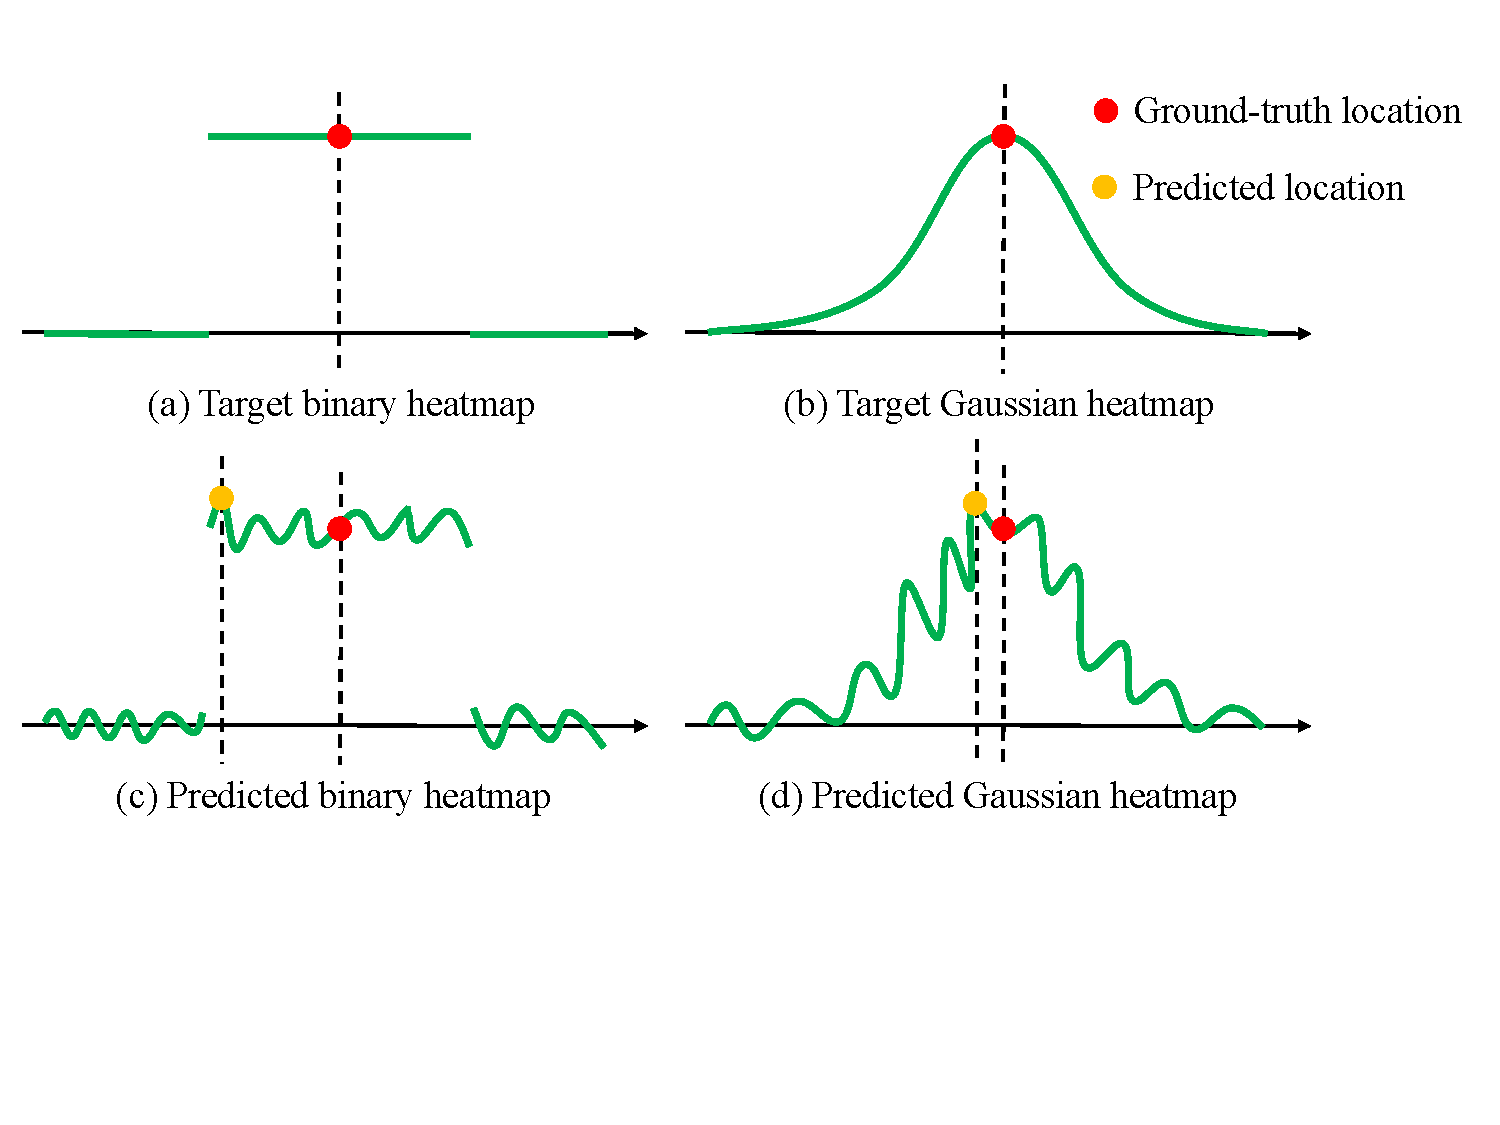
\includegraphics[width=15cm]{multiple_signal_detection/images/heatmap}}
	\caption{Schematics of target and predicted heatmaps. Drawn for a target rectangular distribution (\emph{a}, \emph{c}) and for a Gaussian distribution (\emph{b}, \emph{d}). Taken from \cite{wang2021lowresolutionhumanposeestimation}.}
	\label{fig:heatmap:rect_vs_gaussian}
\end{figure}

% delta peak not suited
% too sparse, and downsampling complications
% for this reason \cite{PhysRevD.100.063015} uses rect function
% following standard heatmap approach \cite{tompson2014jointtrainingconvolutionalnetwork} we use gaussian
% better time resolution see fig

In order to train models to predict such a heatmap $\hat{H}(t)$, it has to be considered what the ground-truth heatmap $H(t)$ should look like. It is natural to construct the ground truth as zeros everywhere except at the exact signal coalescence times, where a label of one is chosen. From a machine-learning perspective, however, this is problematic: For one, it makes the ground truth heavily imbalanced, which complicates training. Further, the models considered here downsample by a large factor of $256$, and the ground truth has to be downsampled accordingly. Sharp peaks can be lost in that process. (Alternatively, the ground truth could be downsampled with max pooling, but then some amount of time accuracy is lost.)

For these reasons, \cite{PhysRevD.100.063015} employs rectangles of width \SI{0.2}{\second}. However, following standard heatmap regression procedure \cite{tompson2014jointtrainingconvolutionalnetwork}, this work uses Gaussian distributions instead. This choice results in better peak extraction accuracy, as the peak of a Gaussian is clearly defined, which is not the case for a rectangular distribution (see Fig.~\ref{fig:heatmap:rect_vs_gaussian}). The ground truth is constructed from Gaussians with unit amplitude and standard deviation $\sigma=\SI{0.1}{\second}$. The distribution is centered on the corresponding signal coalescence time $t_{\text{coa}}$ and is truncated to a $3\,\sigma$ interval, 
\begin{equation}
	h(t) = \begin{cases}
		\exp{\frac{-(t-t_{\text{coa}})^2}{2\sigma^2}} & \text{if $|t-t_{\text{coa}}|\leq3\sigma$, } \\
		0 & \text{else.}
	\end{cases}
\end{equation}

\begin{figure}
	\centering
	\makebox[\textwidth]{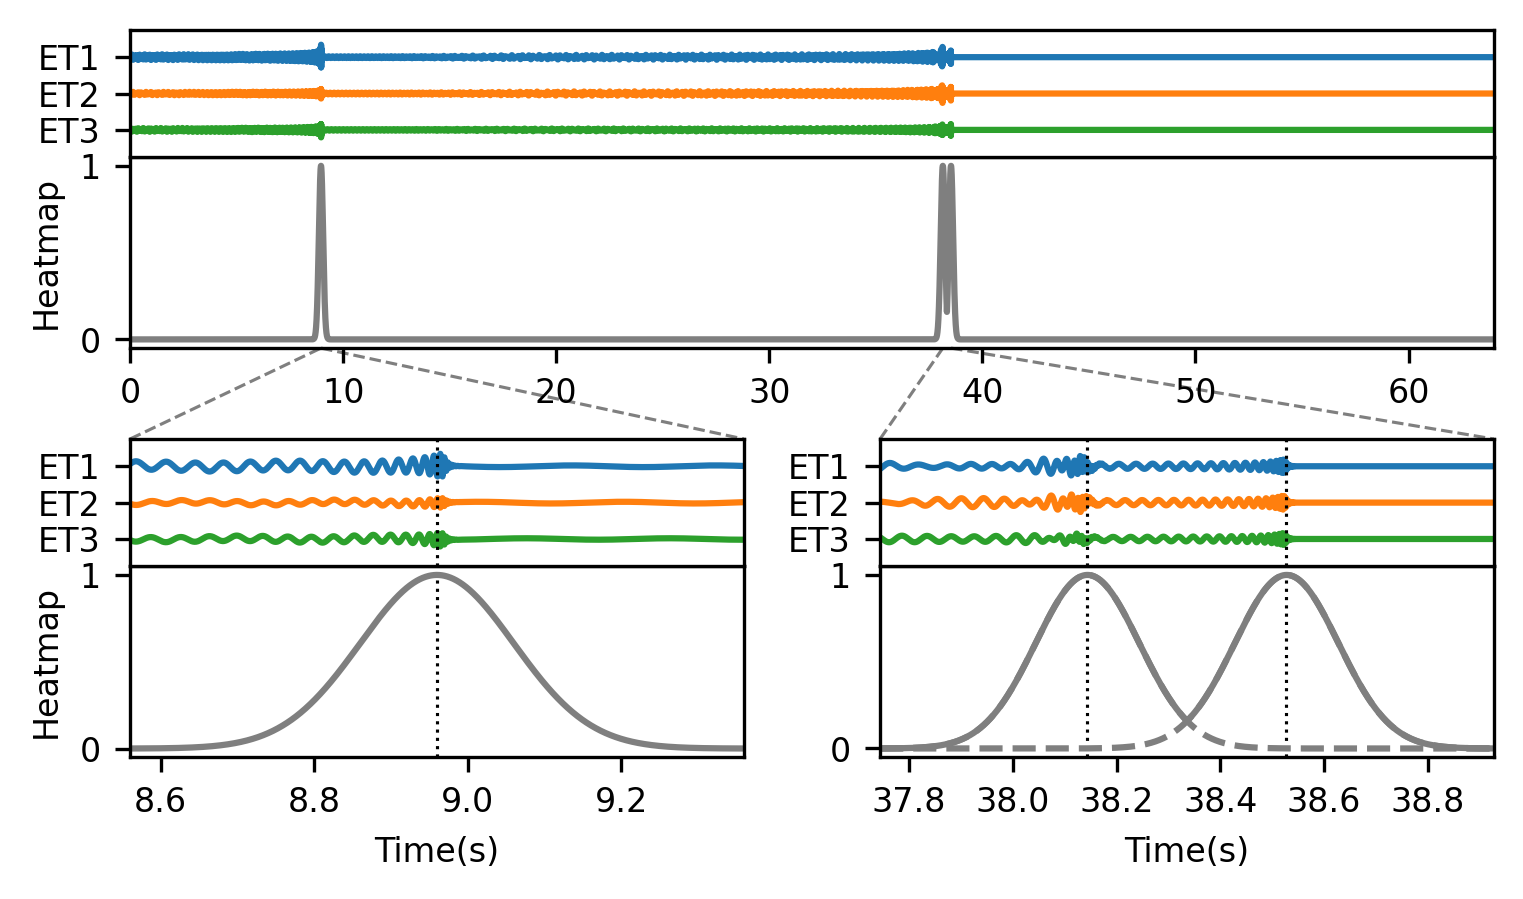
\includegraphics[width=15cm]{multiple_signal_detection/images/heatmap/sample}}
	\caption{Heatmap of a \SI{64}{\second} sample, constructed as the time-wise maximum of multiple Gaussians. Drawn on top of each plot are the individual detector \emph{signal} contributions. For better readability, only the signal and not the full signal + noise strain is shown.}
	\label{fig:heatmap:example_heatmaps}
\end{figure}

% overlapping signals?
% cannot be added up because heatmap has to be in [0,1]
% following \cite{law2019cornernetdetectingobjectspaired}, use max instead
% see fig

From multiple such distributions, a single heatmap could be naively constructed by summing them. However, this can result in heatmap values larger than one, which is impractical for training. Instead, this work follows \cite{law2019cornernetdetectingobjectspaired} and constructs the ground-truth heatmap using a time-wise max operation over all signal distributions, 
\begin{equation}
	H(t) = \max(h_1(t), h_2(t), \dots).
\end{equation}
If a sample contains no signals, $H(t)=0$. See an example heatmap in Fig.~\ref{fig:heatmap:example_heatmaps}.

% postprocessing
% get all peaks with min delta of 1sigma
% score is the peak value
% around each peak estimate sub pixel position according to \cite{bulat2021subpixelheatmapregressionfacial}
% use region of 2 sigma
% softmax
% time is weighted mean

GW candidates are extracted from the predicted heatmap $\hat{H}(t)$ via a peak finding algorithm. All peaks, regardless of height, are extracted. Thresholds are applied later when computing operating points. A minimum distance of \SI{0.1}{\second} is enforced between peaks. For this, methods implemented by SciPy~\cite{2020SciPy-NMeth} are relied upon. 

The extracted peak positions are denoted $x_i$. The GW candidate scores are the peak heatmap values, $\hat{c}_i = \hat{H}(x_i)$. For the corresponding time prediction $\hat{t}_i$, sub-pixel accuracy is achieved with a \emph{soft argmax} operation \cite{bulat2021subpixelheatmapregressionfacial}, which is applied locally around peaks. 

To this end, for each peak $x_i$, the predicted heatmap values outside a $1\,\sigma$ radius are masked. This can be written as,
\begin{equation}
	w_i(t) = \begin{cases} 
		\hat{H}(t) & |t-x_i| < \sigma \\
		-\infty & \text{else.}
	\end{cases}
\end{equation} 
Setting masked values to $-\infty$ will be justified later on. Then, the time-prediction $\hat{t}_i$ is estimated as the soft argmax of $w_i$, 
\begin{equation}
	\hat{t}_i = \sum_t \softmax{(w_i)}(t)\,t.
\end{equation}
% TODO: ugly sentence
The softmax operation, 
\begin{equation}
\softmax{\vec{x}} = \frac{1}{\sum_i \e^{x_i}} \begin{pmatrix}
	\e^{x_0} & \e^{x_1} & \dots & \e^{x_{N-1}}
\end{pmatrix}^\intercal,
\end{equation} 
ensures that the values of $\softmax{(w_i)}(t)$ sum to one and returns zeros outside the considered $1\,\sigma$-radius, where $w_i(t) = -\infty$.

\section{CNN and Transformer Models}

\begin{figure}
	\centering
	\makebox[\textwidth]{
		\includegraphics[width=7.5cm]{multiple_signal_detection/images/heatmap_CNN}
		\hspace{0cm}
		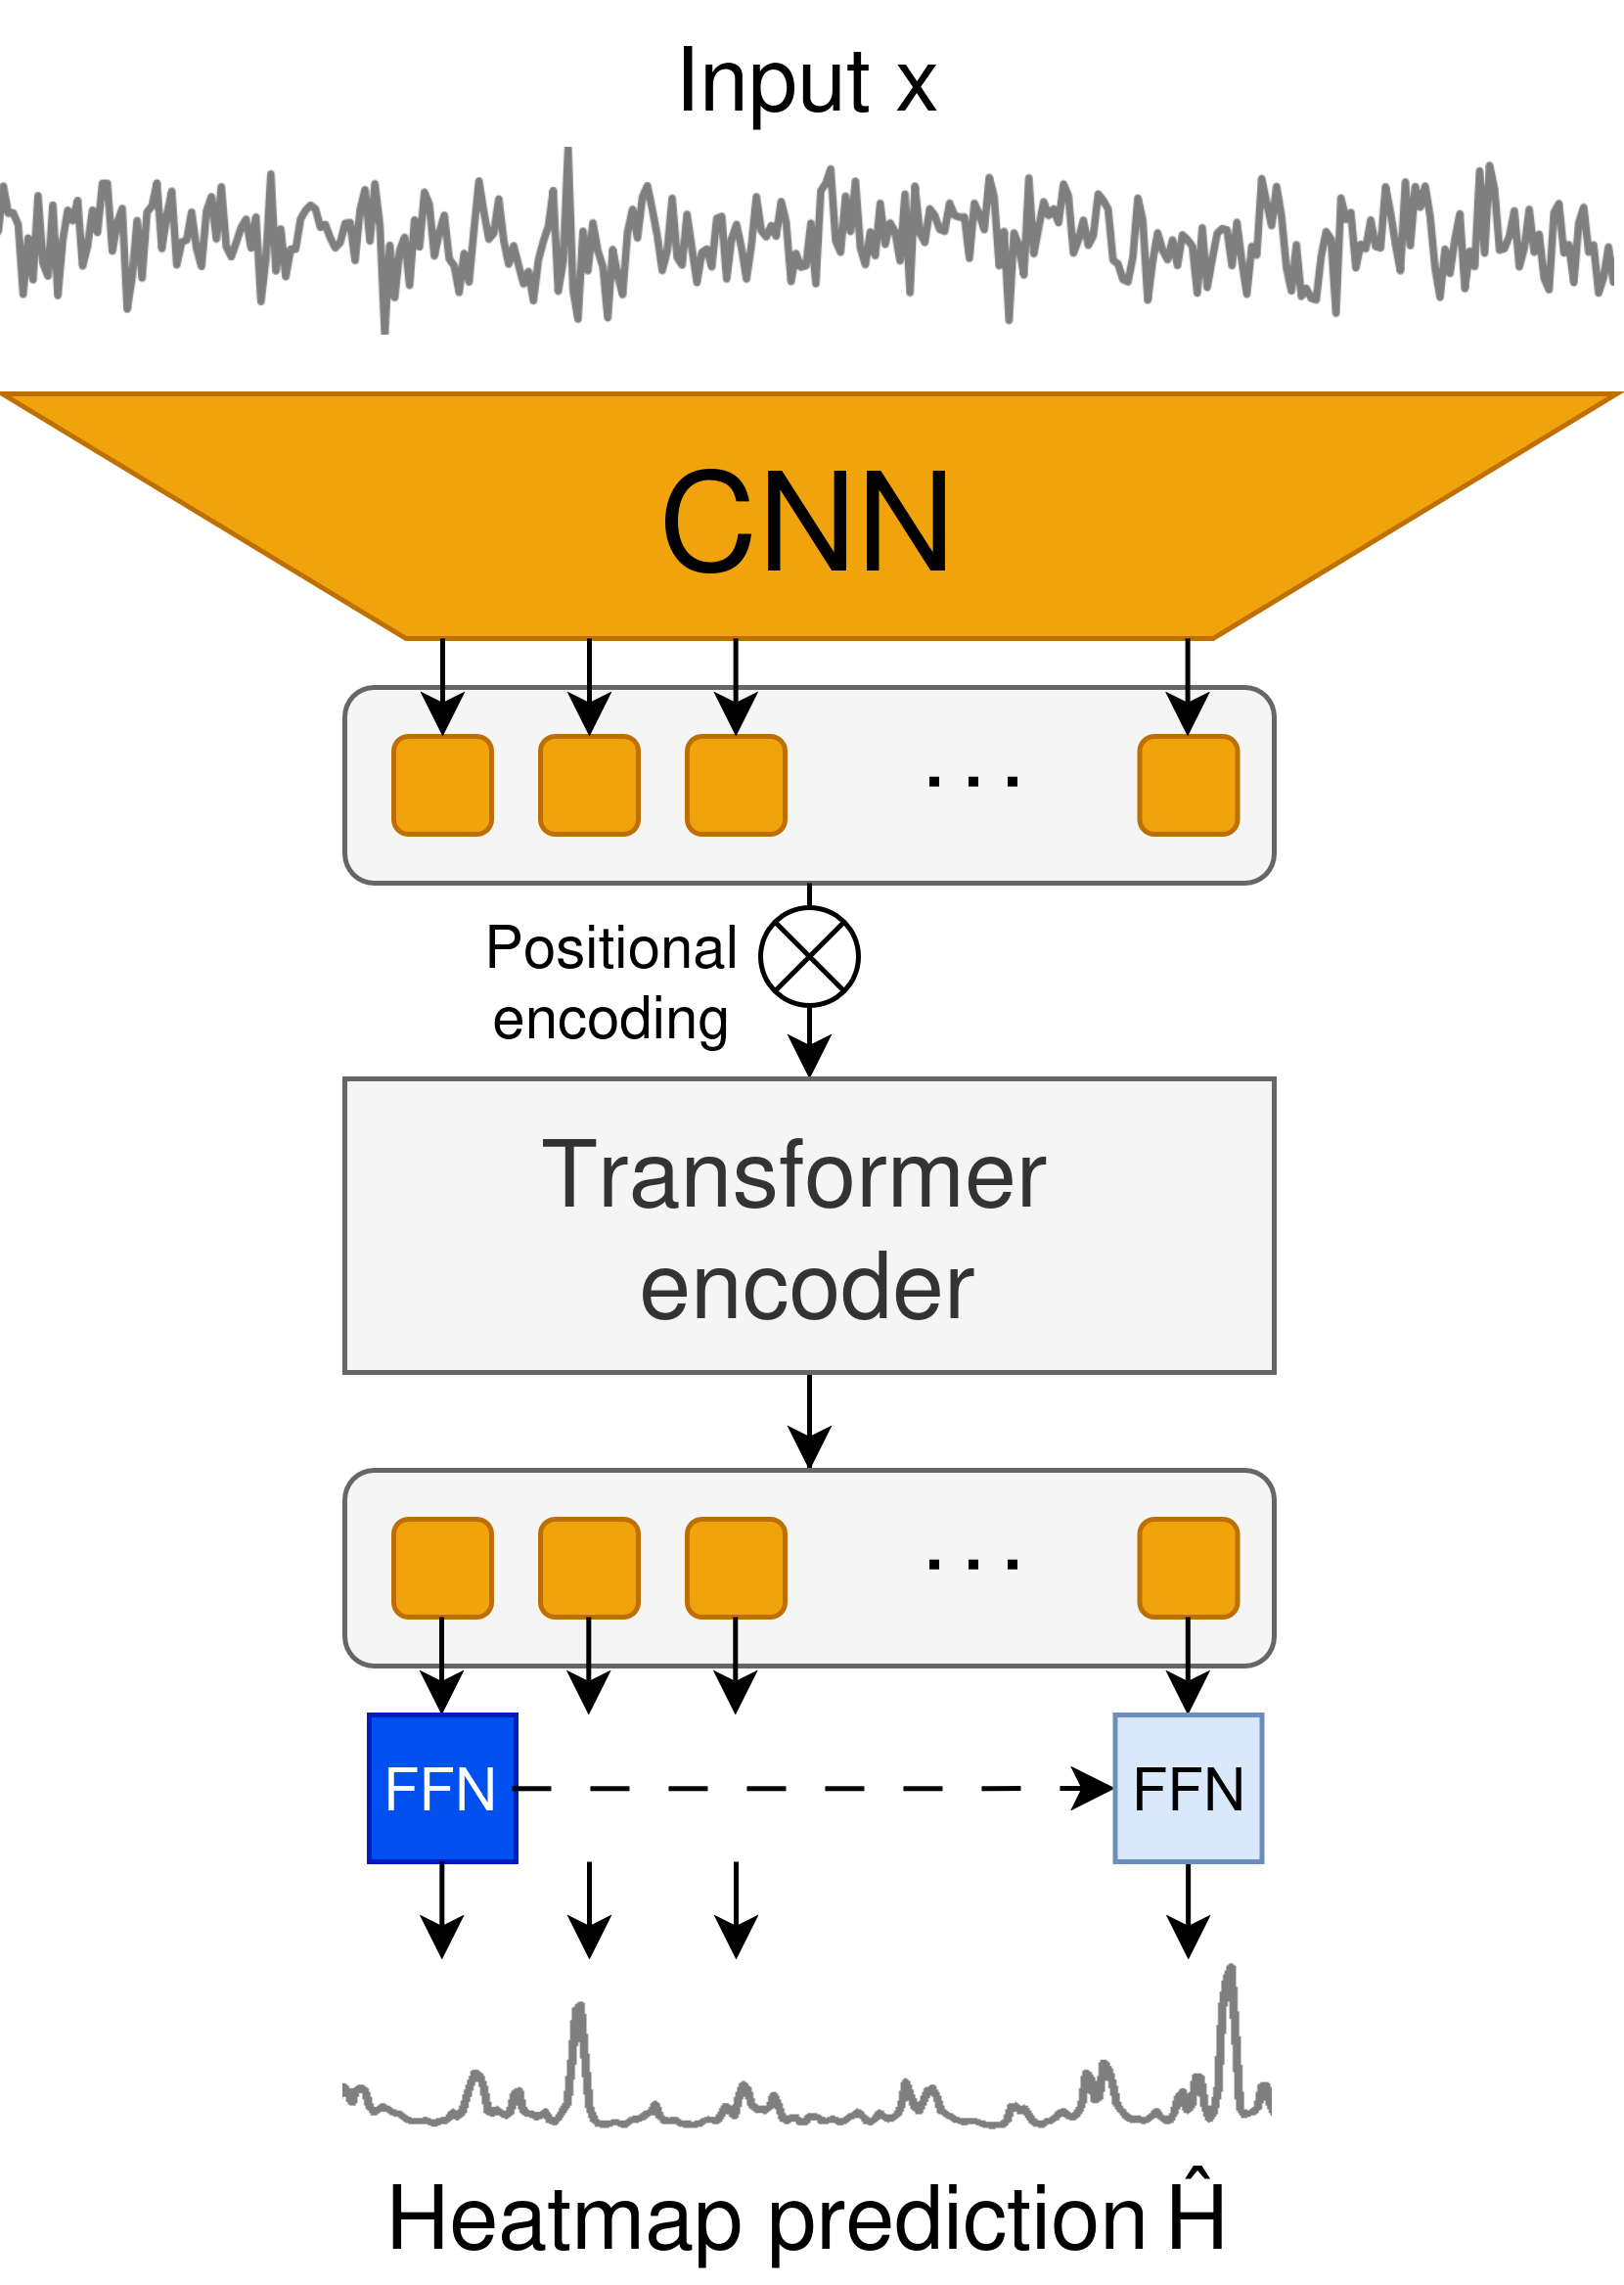
\includegraphics[width=7.5cm]{multiple_signal_detection/images/heatmap_transformer}
	}
	\caption{Schematics of the CNN (\emph{left}) and the transformer encoder (\emph{right}) heatmap regressor models.}
	\label{fig:heatmap:models}
\end{figure}

% two models one cnn and one transformer encoder model with cnn tokenizer
% adjust previous models
% CNN no avg pool and cls head, but sliding cls head
% 700k params
% transformer no cls token, slide cls head over all output tokens
% sinsuoidal pos encondings, embed dim of 64, 8 heads, 6 layers
% 2.2M params

Motivated by the results in \cite{Papalini_2025}, this chapter compares one CNN-based and one transformer-based heatmap regressor. For this, the models implemented in Ch.~\ref{sec:long_duration} are repurposed. The CNN model is the same ResNet model that was presented in the previous chapter. Only the average pooling over the time dimension is discarded. The classification head is then applied over all downsampled time steps to produce a heatmap of length $512$. The classification head is a FFN that takes a vector with $256$ features and returns one number, 
%\begin{equation}
%	\label{eq:heatmap:classification_head}
%	z = \text{Dropout}(\text{Linear}_{1024\rightarrow1}(\text{ReLU}(\text{Dropout}(\text{Linear}_{256\rightarrow1024}(\text{BatchNorm}(x))))))
%\end{equation}
\begin{equation}
\begin{aligned}
	\label{eq:heatmap:classification_head}
	n &= \mathrm{BatchNorm}(x),\\
	h &= \mathrm{Dropout}(\mathrm{ReLU}(\mathrm{Linear}_{256\rightarrow1024}(n))),\\
	z &= \mathrm{Dropout}(\mathrm{Linear}_{1024\rightarrow1}(h)),
\end{aligned}
\end{equation}
with a dropout probability of \SI{10}{\percent}. The output is later passed through a sigmoid activation to yield heatmap values in $[0,1]$. The model has a total of \SI{700}{\kilo\nothing} parameters. Apart from the exact implementation of the CNN and classification head, this architecture is the same as \cite{PhysRevD.100.063015}.

Similar to the ViT, the transformer model considered here consists of a transformer encoder only. The model uses the same ResNet for tokenization, again, resulting in $512$ tokens with embedding dimension $d_\text{embed}=64$. Instead of appending a single classification token, \emph{all} encoder output tokens are fed through a classification head. This is an FFN similar to Eq.~\ref{eq:heatmap:classification_head} with an input size of $64$ instead, and yields a heatmap of length $512$. The model employs sinusoidal positional encodings, and the encoder consists of six layers and eight heads. The transformer FFNs have $d_\text{ff}=1024$. A dropout probability of \SI{10}{\percent} is used throughout. The total number of trainable parameters is \SI{2.2}{\mega\nothing}. See schematics of both the CNN and transformer encoder models in Fig.~\ref{fig:heatmap:models}. 

% training is complicated by positive label sparsity
% use time-wise bce loss, weighting positive label by a large factor of 0.98
% (often in heatmap regression, more complicated losses are used because element-wise losses cannot appropriately measure the difference between distributions) 

The model weights are optimized by minimization of the time-wise BCE loss of the ground truth and predicted heatmap $H(t)$ and $\hat{H}(t)$. For ground-truth labels continuous in $[0,1]$, this is defined as,
\begin{equation}
	\pazocal{L}_\text{BCE}(H(t), \hat{H}(t)) = -(\alpha H(t) \ln{\hat{H}(t)} + (1 - \alpha) (1-H(t)) \ln{(1-\hat{H}(t))}).
\end{equation}
Because of label sparsity, the loss term corresponding to positive labels is up-weighted by a factor $\alpha$ and the other term down-weighted by $(1-\alpha)$. For this, a relatively high positive-label weight of $\alpha = 0.98$ is chosen empirically. In practice, this loss is calculated from the pre-sigmoid logits.

% AdamW lw 1e-4 weightdecay 1e-4
% CNN reduce on plateau (factor: 0.1, patience: 15, threhsold: 0.01)
% cosine annealing with warmup of 5000 steps

Models are trained for a maximum of $100$ epochs using the AdamW optimizer with a learning rate of \SI{E-4}{\nothing} and a weight decay of \SI{E-4}{\nothing}. The batch size is $64$. For the CNN model, the learning rate is reduced by a factor $0.1$ if the validation loss does not decrease by at least $0.01$ over $15$ epochs. The encoder model is trained with a cosine-annealing schedule with a warmup of $5000$ steps. 

\begin{figure}
	\centering
	\makebox[\textwidth][c]{%
		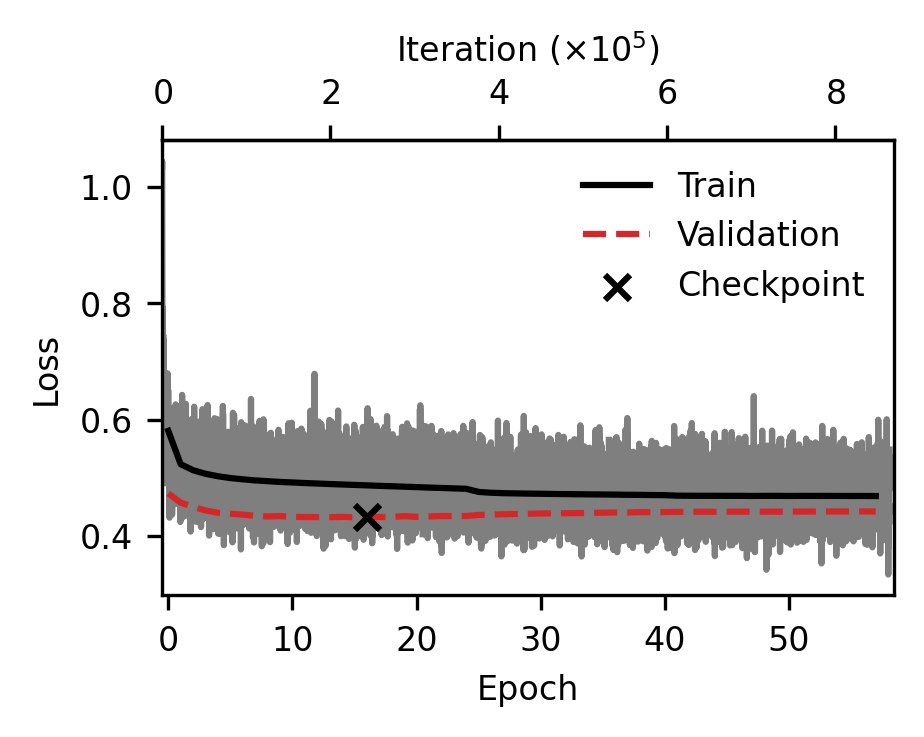
\includegraphics[width=8cm]{multiple_signal_detection/plots/learning_curves/cnn_loss}%
		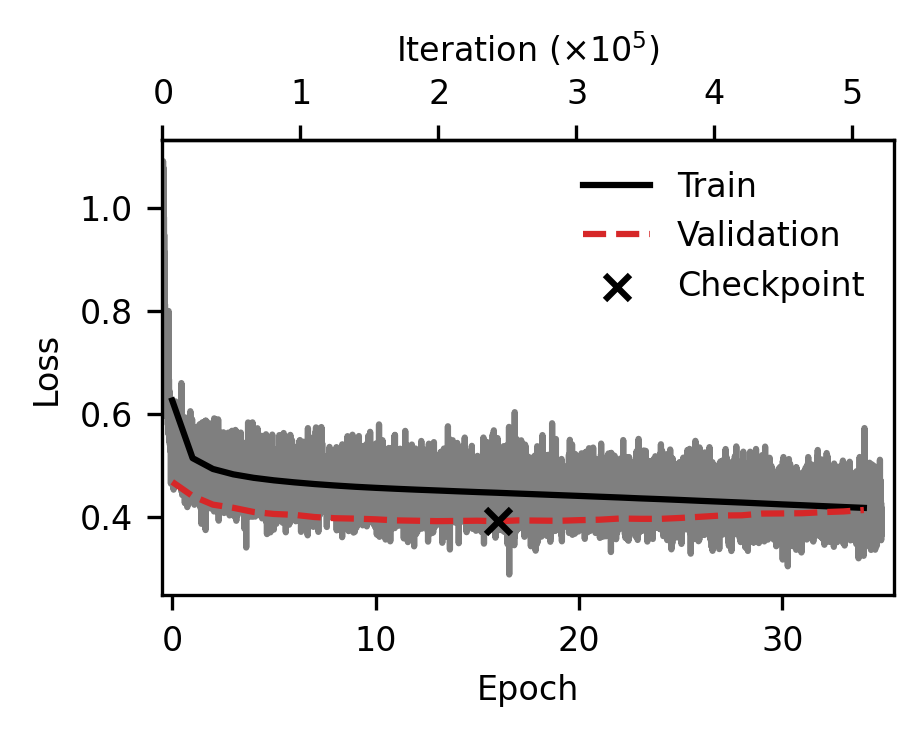
\includegraphics[width=8cm]{multiple_signal_detection/plots/learning_curves/encoder_loss}
	}
	\caption{Learning curves of the CNN (\emph{left}) and the encoder model (\emph{right}). The training loss is plotted for each step (\emph{grey}) and as averaged over all steps in one epoch (\emph{black}). The validation loss is plotted in red and a marker signifies its minimum.}
	\label{fig:heatmap:learning_curves}
\end{figure}

% see learning curve in fig
% similar to the vit learning curves, the plot shows lower validation loss because of final dropout layer

See both learning curves in Fig.~\ref{fig:heatmap:learning_curves}. Both models start to overfit after $16$ epochs. Similar to the ViT learning curves, the plot shows a lower validation loss in the early epochs because of the classification head's final dropout layer.

\section{Performance Comparison}

\begin{figure}
	\centering
	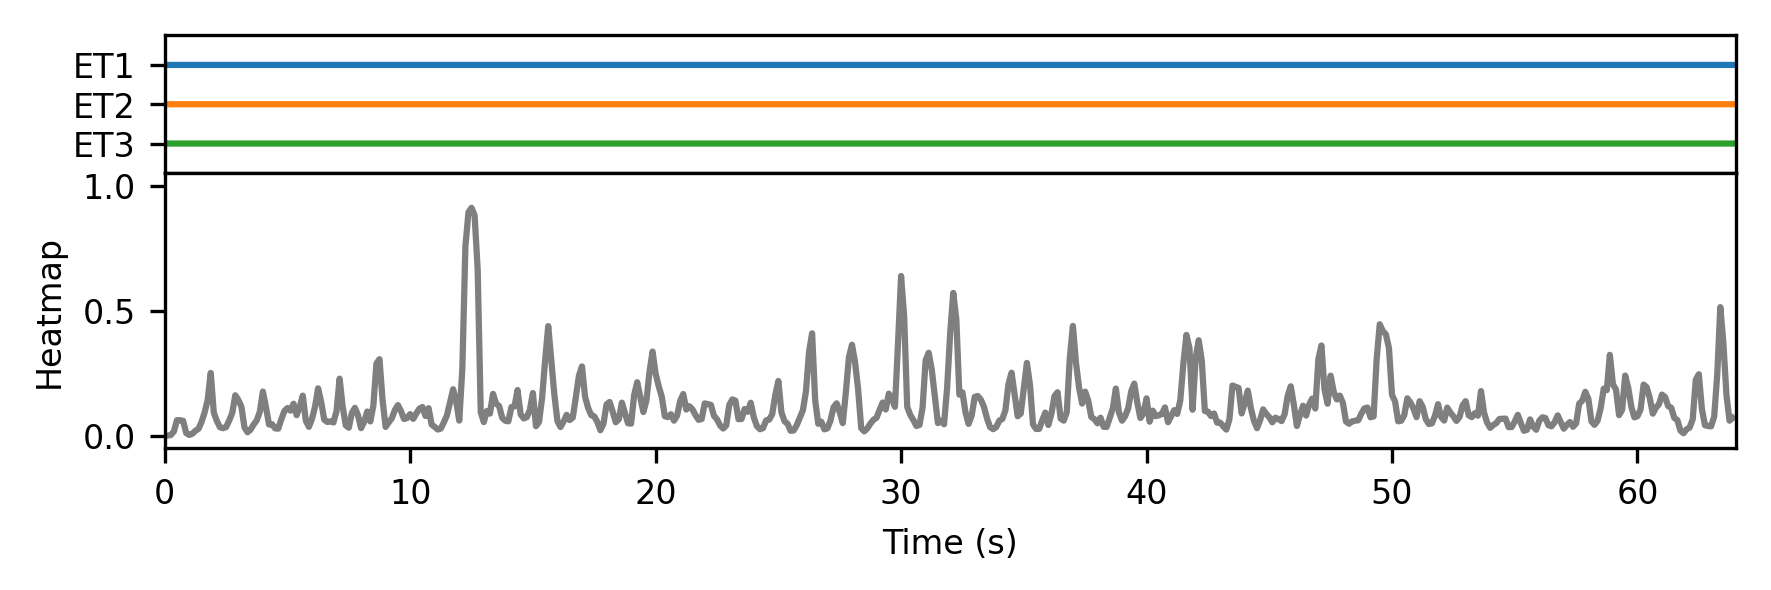
\includegraphics[
	width=15cm,
	trim=0 1cm 0 0,
	clip
	]{multiple_signal_detection/plots/out/300/encoder/11}
	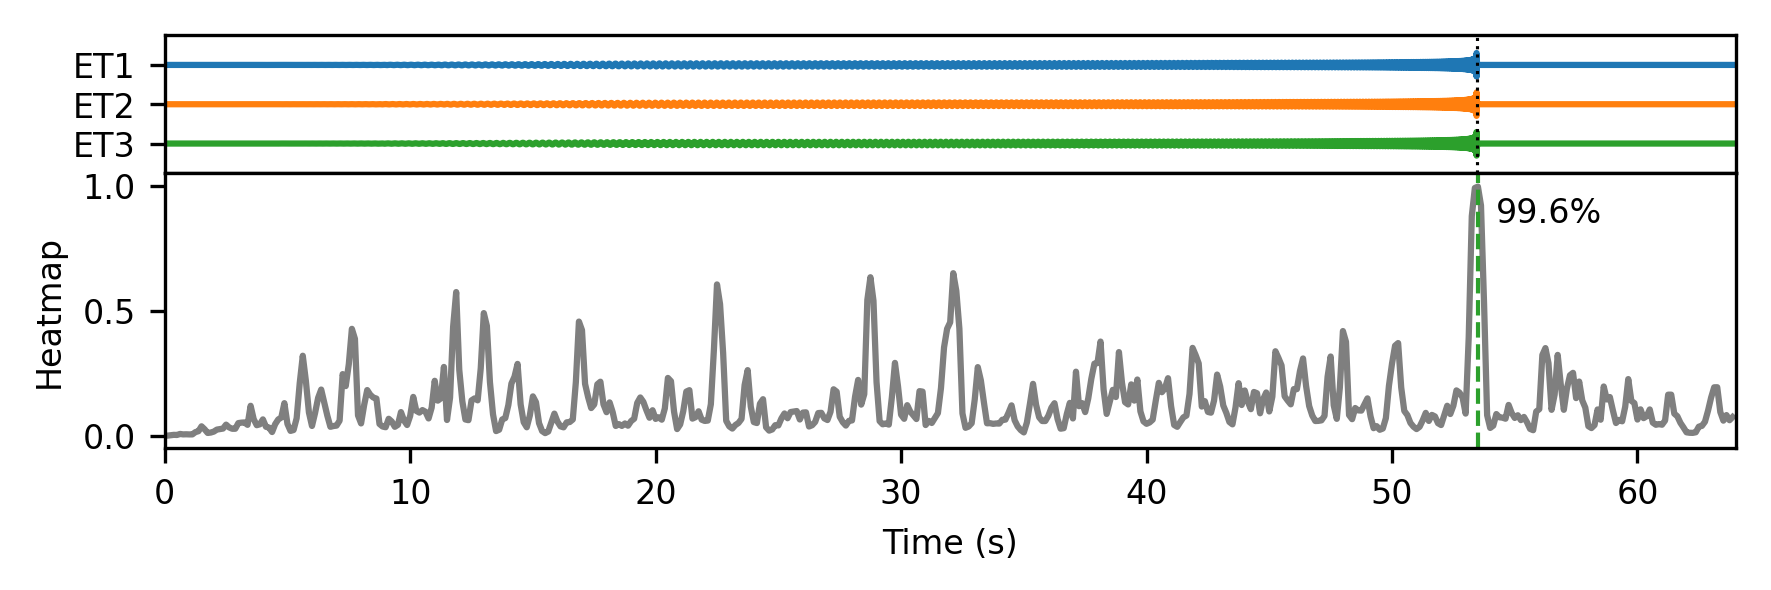
\includegraphics[
	width=15cm,
	trim=0 1cm 0 0,
	clip
	]{multiple_signal_detection/plots/out/300/encoder/1}
	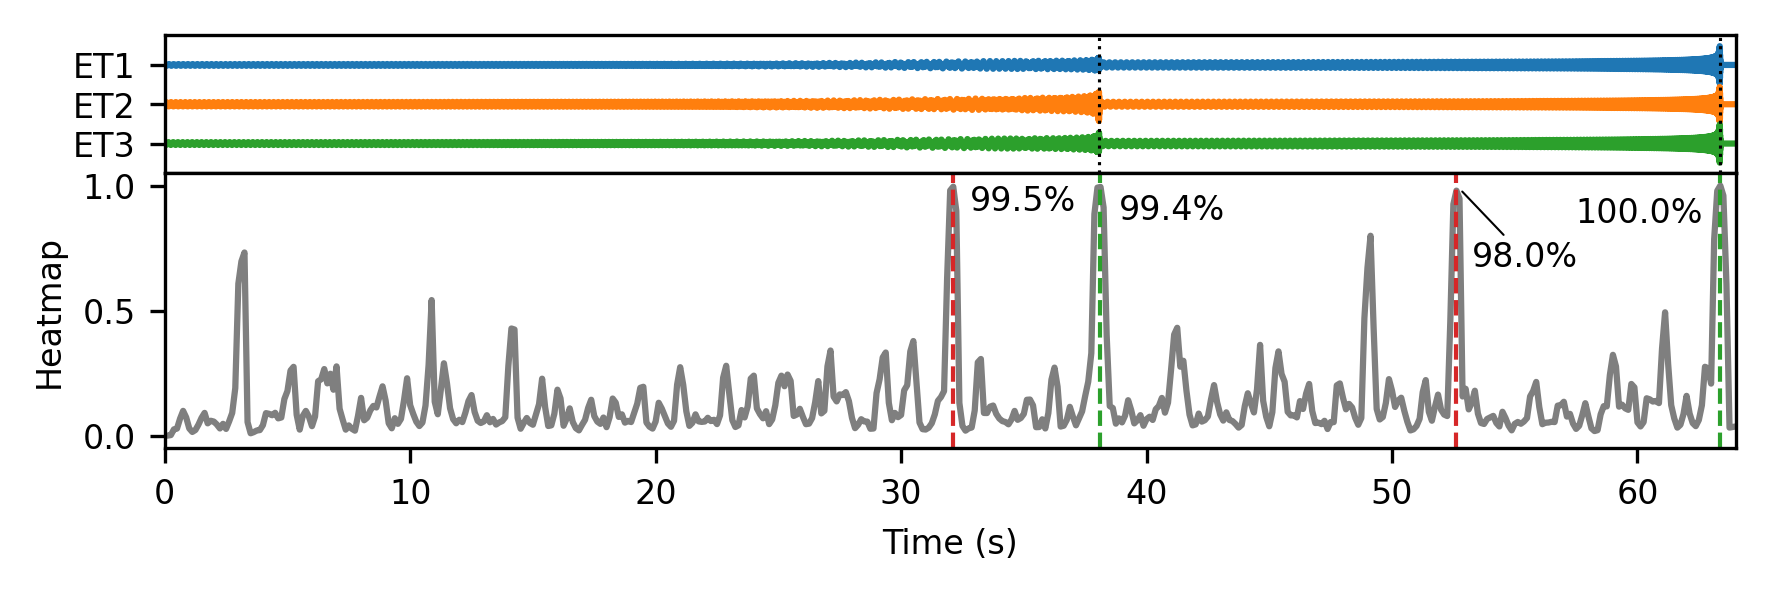
\includegraphics[
	width=15cm,
	trim=0 1cm 0 0,
	clip
	]{multiple_signal_detection/plots/out/300/encoder/3}
	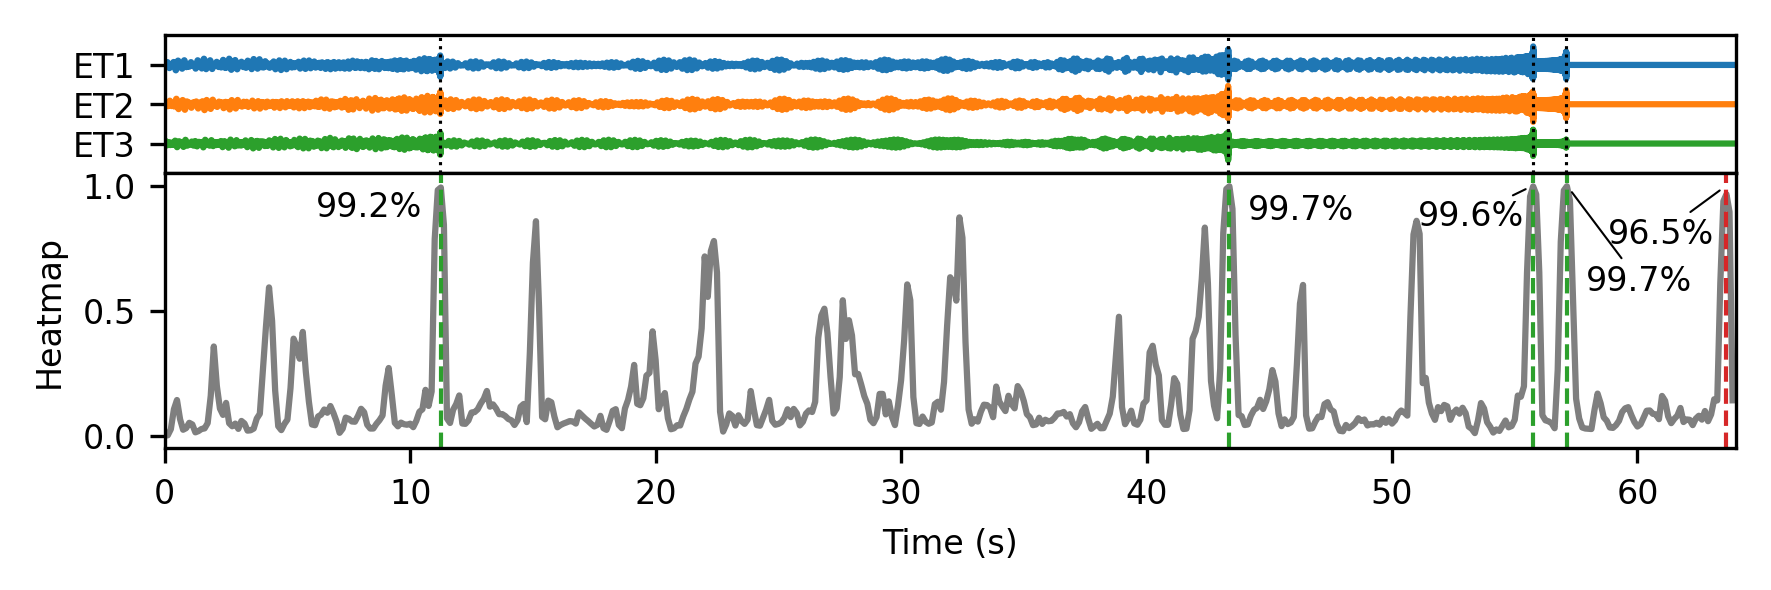
\includegraphics[
	width=15cm,
	trim=0 1cm 0 0,
	clip
	]{multiple_signal_detection/plots/out/300/encoder/0}
	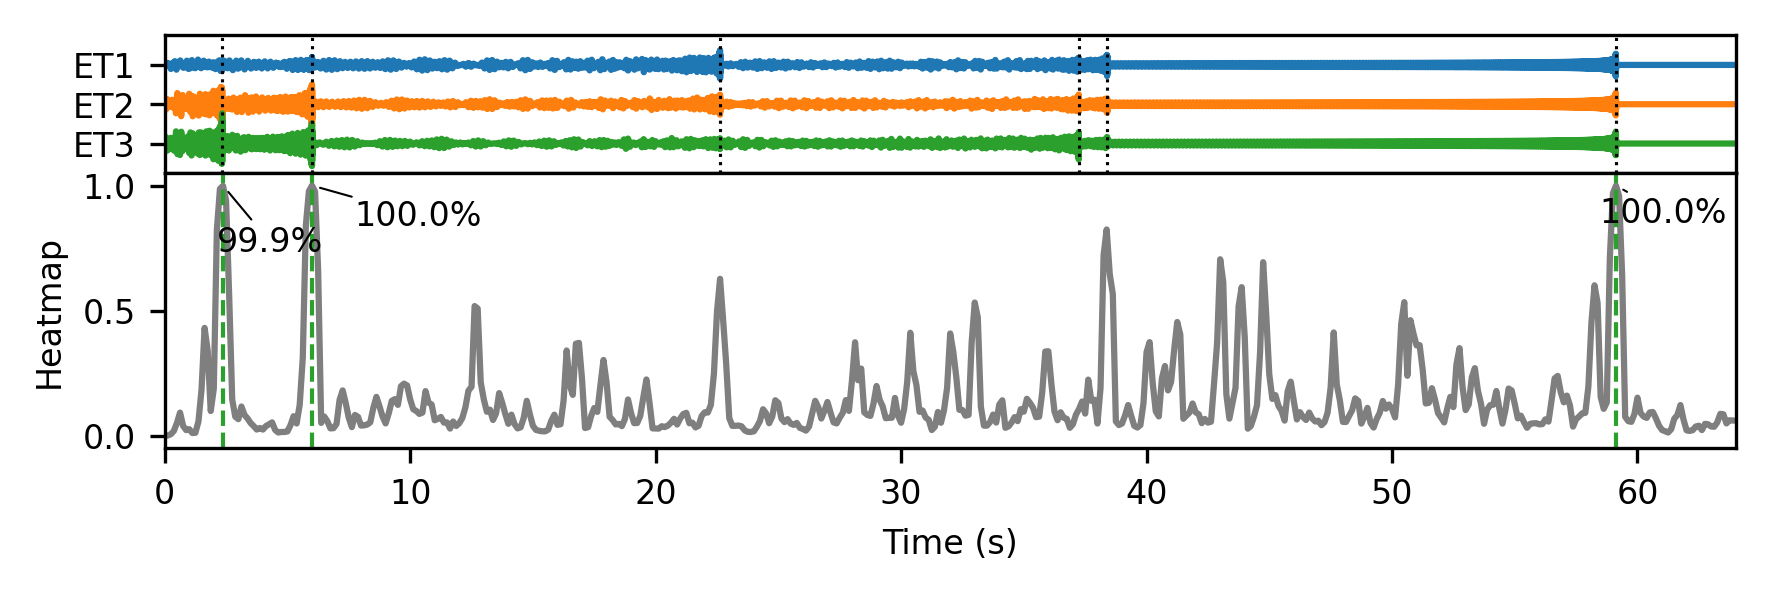
\includegraphics[
	width=15cm,
	]{multiple_signal_detection/plots/out/300/encoder/8}
	\caption{Predicted heatmaps for five samples produced by the encoder model. Peaks above a threshold of \SI{96}{\percent} are GW candidates. For each candidate, the class score is indicated and the time prediction is shown as a vertical line. This line is colored green for TPs and red for FPs.}
	\label{fig:heatmap:encoder_out}
\end{figure}

% get a sense of whats going on see fig
% network is quite trigger happy -> high positive weight
% still when using a high threshold of 96.0%, most signals can be retrieved while not producing too many FPs (the choice of this threshold will justified soon)
% The time resolution seems too be sufficient. In these 5 example samples, no prediction is labeled FP because it differs more than 0.1s from the correspondiing merger

Before evaluating the models quantitatively, it is useful to inspect individual predicted heatmaps. Fig.~\ref{fig:heatmap:encoder_out} shows the transformer encoder model's output for five test samples. It can be seen that the model is quite trigger-happy, producing $\approx100$ peaks per sample. This behavior is expected to some extent, as the models were trained with a high positive weight. Still, by employing a relatively high score threshold of \SI{96}{\percent}, most signals can be retrieved without producing too many FPs. (The exact value of that threshold depends on the desired FAR. This will be covered later.) Further, it appears that the predicted time resolution is sufficient for the chosen matching criterion: In the examples shown, no prediction is labeled FP because the time prediction differs by more than \SI{0.1}{\second} from the ground-truth signal coalescence time.

\begin{figure}
	\centering
	\makebox[\textwidth]{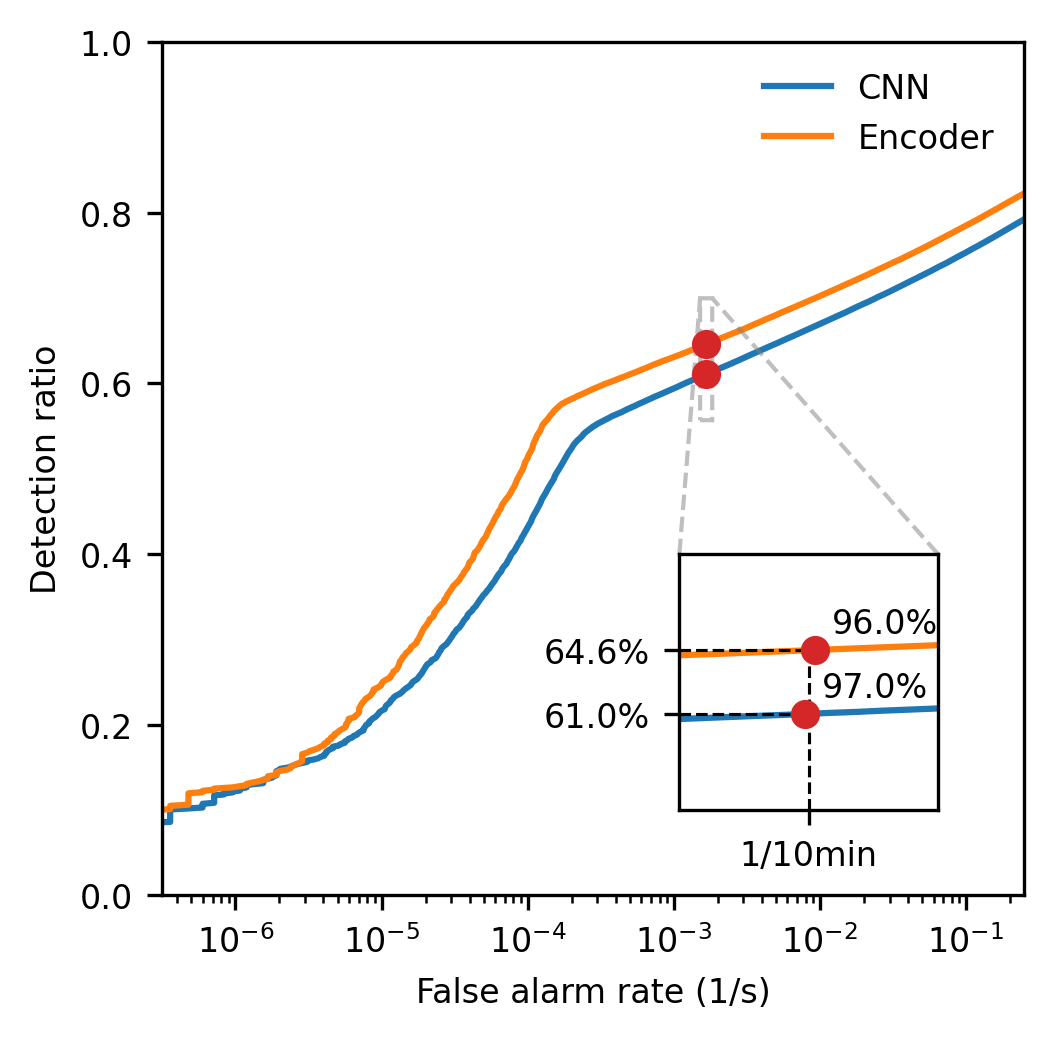
\includegraphics[width=9cm]{multiple_signal_detection/plots/cnn_encoder_far}}
	\caption{Detection ratio as a function of FAR for the CNN (\emph{blue}) and transformer encoder (\emph{orange}) models. Computed over  \SI{131}{\kilo\nothing} test samples containing \SI{393}{\kilo\nothing} signals. The upper FAR limit corresponds to $16$ FPs per sample, and the lower limit is $1/\SI{}{\month}$. Markers indicate the fixed operating points, where $\text{FAR}=1/\SI{10}{min}$. For each marker, the corresponding threshold is written out. Uncertainties are too small to be visualized.}
	\label{fig:heatmap:encoder_far}
\end{figure}

% more robust way of estimating performance, also too compare cnn and encoder model
% plot operating characteristic of FAR, detection ratio for different thresholds
% see the results in fig
% models reach quite low FAR of 1/month while retaining some amount of signals (10% to 20%)

A robust performance test is obtained by varying the score threshold and computing the detection ratio and FAR over the whole test dataset. The detection ratio is computed over \SI{393}{\kilo\nothing} signals. This gives a maximum uncertainty of \SI{0.08}{\percent}, assuming a binomial distribution\footnote{Strictly speaking, this assumption is wrong, as trials are not independent when dealing with overlapping signals. In particular, it will become clear that the detection ratio decreases for closely separated signals. Still, the results will show that this effect is only relevant for signals with separations $\leq\SI{0.6}{\second}$, which does not amount to a large number of signals. Thus, the binomial uncertainty still serves as a useful estimate.}. The operating characteristics for the CNN and transformer encoder models are shown in Fig.~\ref{fig:heatmap:encoder_far}. Both models reach low FARs while retaining a non-zero fraction of signals. At a FAR of $1/\SI{}{\month}$, the detection ratio is $\approx\SI{10}{\percent}$. The encoder model performs better over the whole FAR range shown in Fig.~\ref{fig:heatmap:encoder_far}. 

To evaluate and compare the models' performance, fixed operating points have to be chosen. While low-latency searches usually aim for FARs of $1/\SI{}{\month}$, the models here do not perform particularly well in this regime. For the purposes of this study, a FAR of $1/\SI{10}{\minute}$ is employed instead, which corresponds to approximately one FP every ten samples. At the corresponding operating points, the models achieve good performance, while not producing too many FPs. For this, the threshold is set to \SI{97.0}{\percent} for the CNN and to \SI{96.0}{\percent} for the encoder model. The CNN reaches a detection ratio of \SI{61.04(8)}{\percent}, while the transformer encoder reaches \SI{64.61(8)}{\percent}. 

At this point, it is natural to ask how this performance compares to matched filtering. A direct comparison is not attempted here because implementing a full matched-filtering search goes beyond the scope of this thesis. Moreover, a quantitative comparison to existing research is complicated by the fact that the datasets used can differ significantly:
\begin{itemize}
	\item For one, studies often employ the lower event-rates of second-generation detectors. It has been shown that for strongly time-overlapping signals, the performance of matched filtering decreases \cite{Relton_2022}. Because of ET's higher event-rate, these overlaps occur frequently in this work's simulations.
	\item Datasets differ in the chosen signal parameters. This matters especially for the component masses, as Ch.~\ref{sec:long_duration} showed that model performance depends strongly on these.
	\item Most importantly, datasets differ in the considered signal SNR. In this work, the SNR is sampled uniformly in $[5,15]$. Studies often sample the distance from a second order power law instead, resulting in a non-uniform SNR distribution. For example, \cite{Relton_2022} reports SNRs up to $50$, which is much louder than this work's test dataset.
\end{itemize}
For these reasons, comparisons to matched filtering will be qualitative in the following. As a rough estimate, offline searches~\cite{Nitz_2017, Relton_2022} reach close to perfect detection ratios for signal SNRs larger than $10$ to $15$ and at FARs $<1/\SI{}{\year}$. For the SNR range considered here, this very loosely translates to a detection ratio of \SI{50}{\percent}. Online searches~\cite{Nitz_2018} reach comparable performance at a FAR of $1/\SI{}{\month}$. Compare this to the detection ratio of $\approx\SI{10}{\percent}$ at a FAR of $1/\SI{}{\month}$, reached by the models here.

\begin{figure}
	\centering
	\makebox[\textwidth]{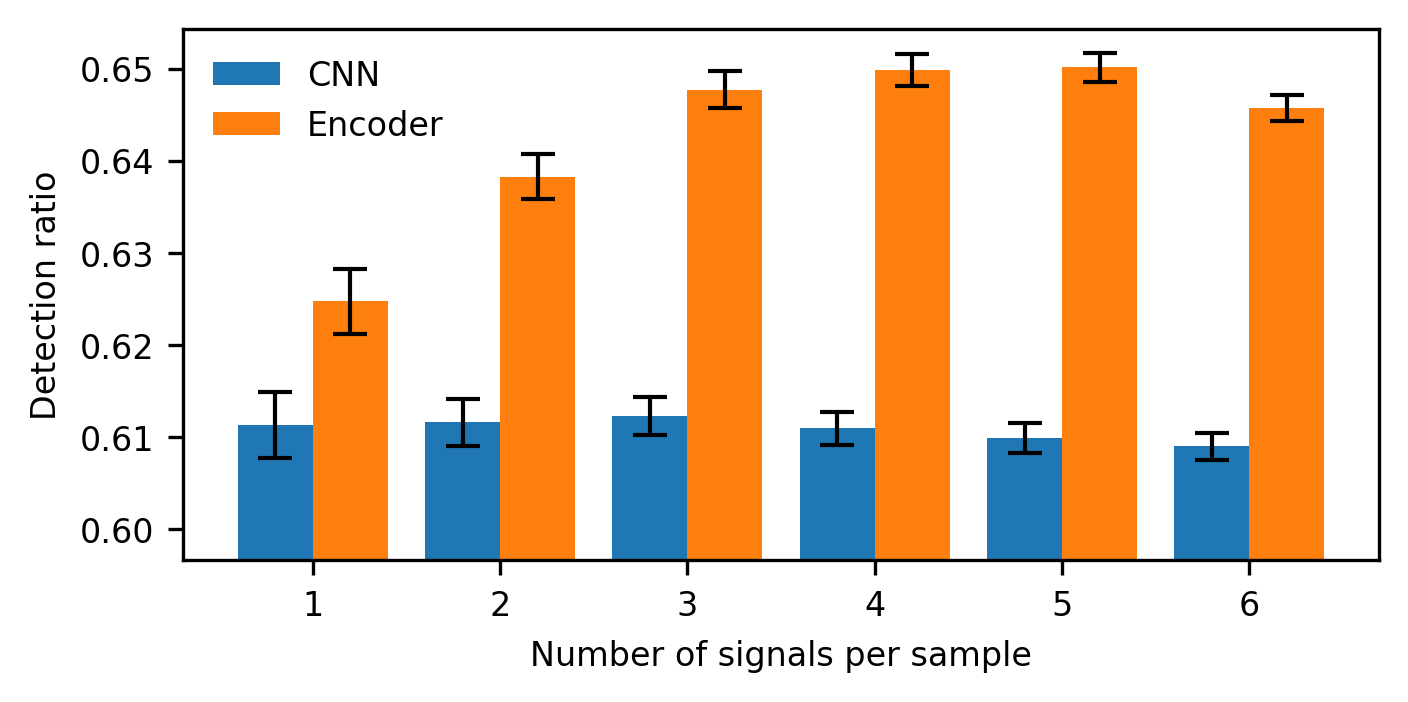
\includegraphics[width=12cm]{multiple_signal_detection/plots/cnn_encoder_mergers}}
	\caption{Detection ratio as a function of $n$, the number of signals per sample, for the CNN (\emph{blue}) and the encoder model (\emph{orange}). Computed over $\SI{19}{\kilo\nothing}$ samples each. The number of signals per sample can be taken as a measure of signal overlap.}
	\label{fig:heatmap:num_mergers}
\end{figure}

% \cite{Papalini_2025} report transformers being good for overlapping signals
% check detection ratio as a function of signals per sample
% see plot
% similar performance if one signals per sample
% CNN decreases for more signals
% interestingly, encoder slightly increases in performance

The results so far show that the transformer model outperforms the conventional CNN approach. Motivated by \cite{Papalini_2025}, it is tempting to attribute this result to the increased signal overlap in the data. This can be tested by examining the detection ratio (at the fixed operating points defined earlier) as a function of the number of signals per sample $n$. Since the sample size is \SI{64}{\second}, multiple signals, $n>1$, will almost always overlap. For this, the test dataset is binned with $n\in[1,6]$ resulting in six subsets of \SI{19}{\kilo\nothing} samples each. These contain \SI{19}{\kilo\nothing}, \SI{37}{\kilo\nothing}, \dots signals, respectively. For each subset, the detection ratio is computed separately, assuming a binomial distribution for the uncertainty. See the results in Fig.~\ref{fig:heatmap:num_mergers}.

The plot shows that both models perform similarly if there is only one signal per sample $n=1$. For increasing $n$, the CNN model stays mostly constant in performance as the detection ratio decreases by $\SI{0.3(3)}{\percent}$ only.
Interestingly, the transformer encoder's detection ratio \emph{increases} by $\SI{2.5(4)}{\percent}$ instead. Thus, the performance difference stems mainly from those samples with multiple overlapping signals: not because increased overlap degrades the CNN performance, but because the encoder improves with more signals per sample.

This difference is likely explained by the models' \emph{receptive fields}. For the CNN, at each time step, the classification head can only attend to $\approx\SI{1}{\second}$ of data. In contrast, in the  transformer encoder model, the classifier can attend to the whole input time series through the \emph{attention mechanism}.
As the CNN does not degrade in performance, it can be argued that its small local receptive field of $\approx\SI{1}{\second}$ is sufficient for capturing signal overlap. This is consistent with \cite{Relton_2022}, where overlap only becomes problematic for signals with coalescence times separated by $<\SI{1}{\second}$. The effect of signal separation on model performance is studied more closely in the following sub-chapter.

\begin{figure}
	\centering
	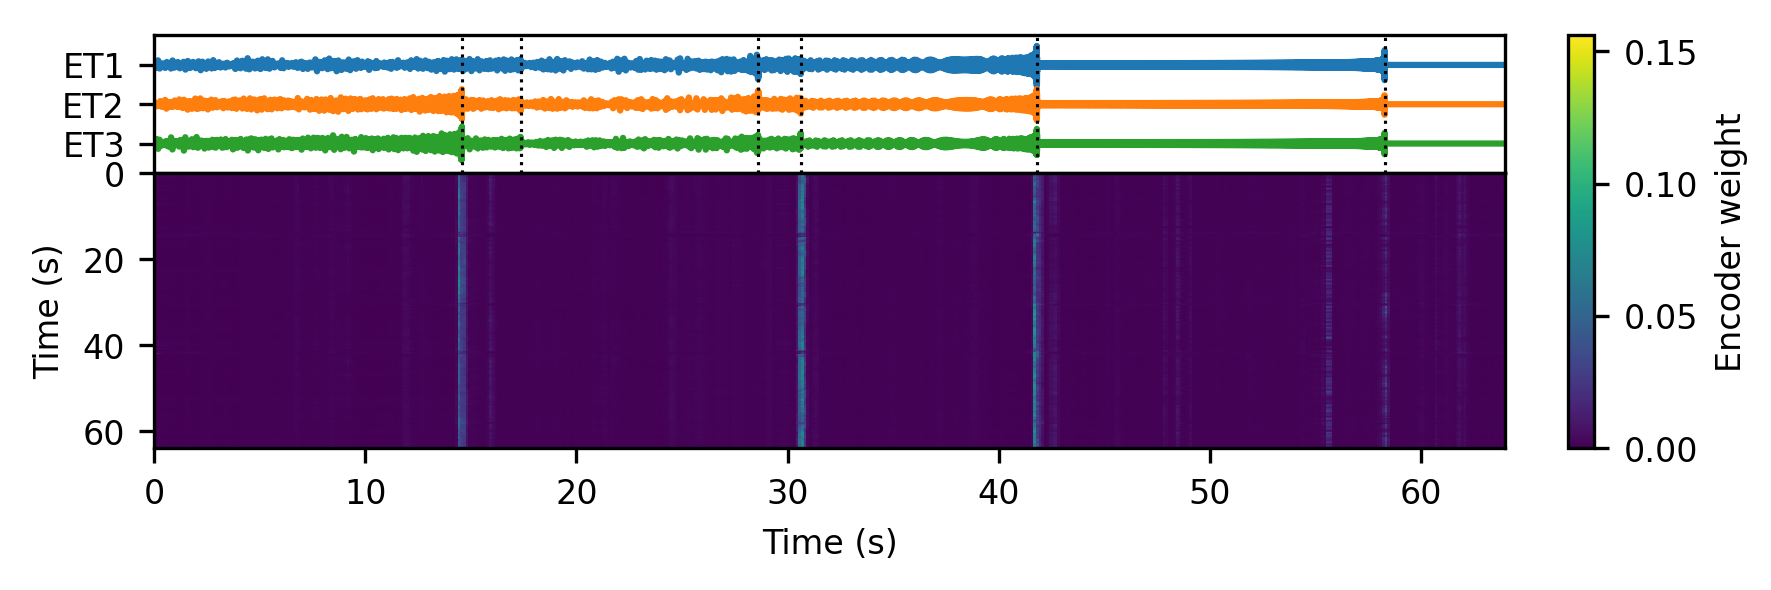
\includegraphics[
	width=15cm,
	trim=0 1cm 0 0,
	clip
	]{multiple_signal_detection/plots/weights/encoder/11}
	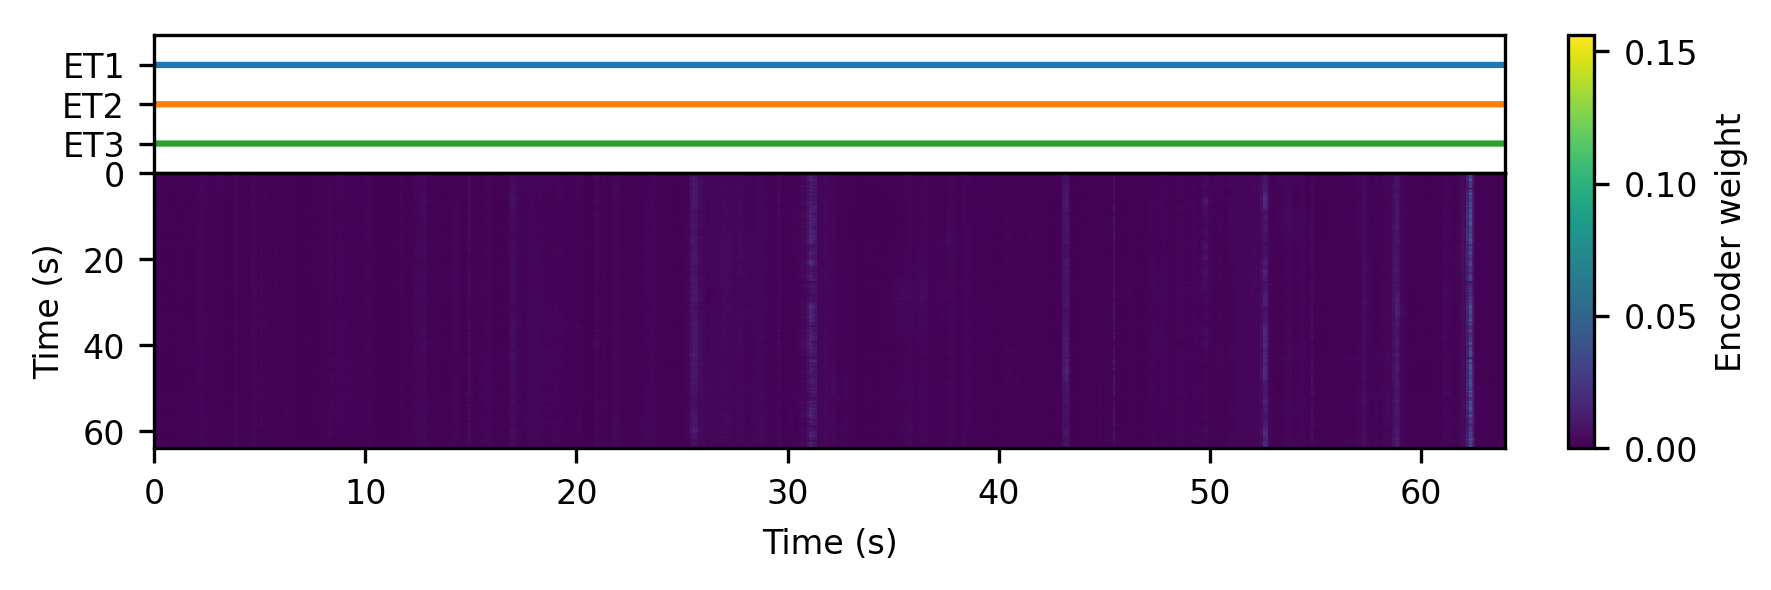
\includegraphics[
	width=15cm,
	trim=0 1cm 0 0,
	clip
	]{multiple_signal_detection/plots/weights/encoder/1}
	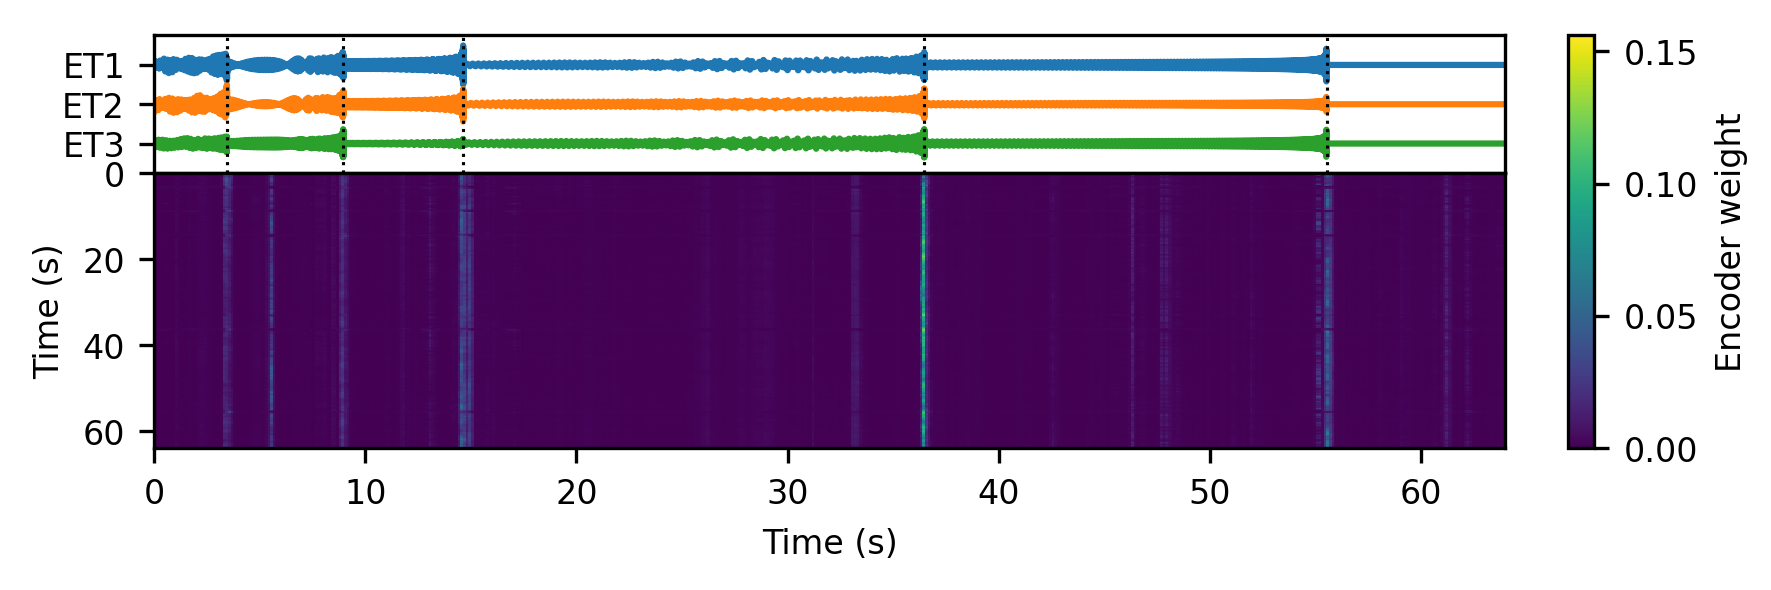
\includegraphics[
	width=15cm,
	trim=0 1cm 0 0,
	clip
	]{multiple_signal_detection/plots/weights/encoder/3}
	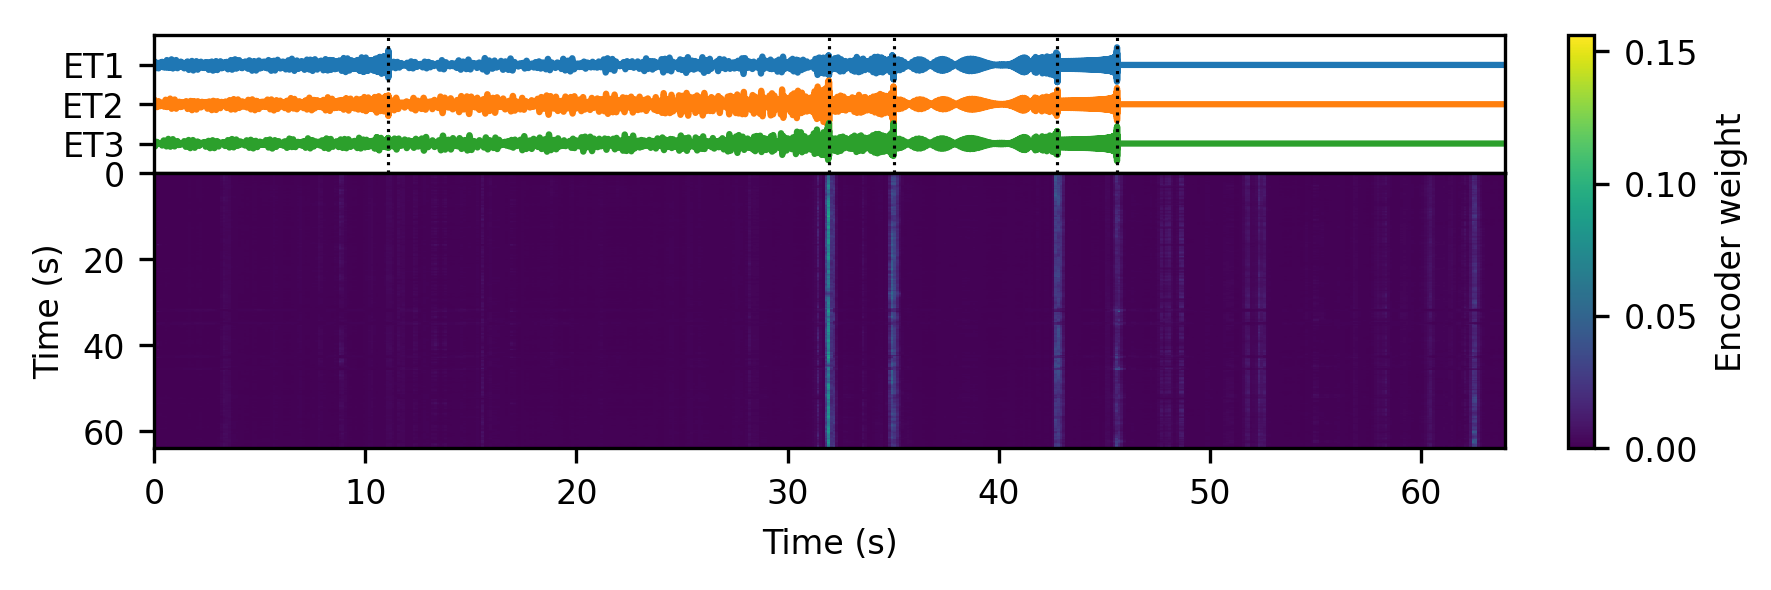
\includegraphics[
	width=15cm,
	trim=0 1cm 0 0,
	clip
	]{multiple_signal_detection/plots/weights/encoder/0}
	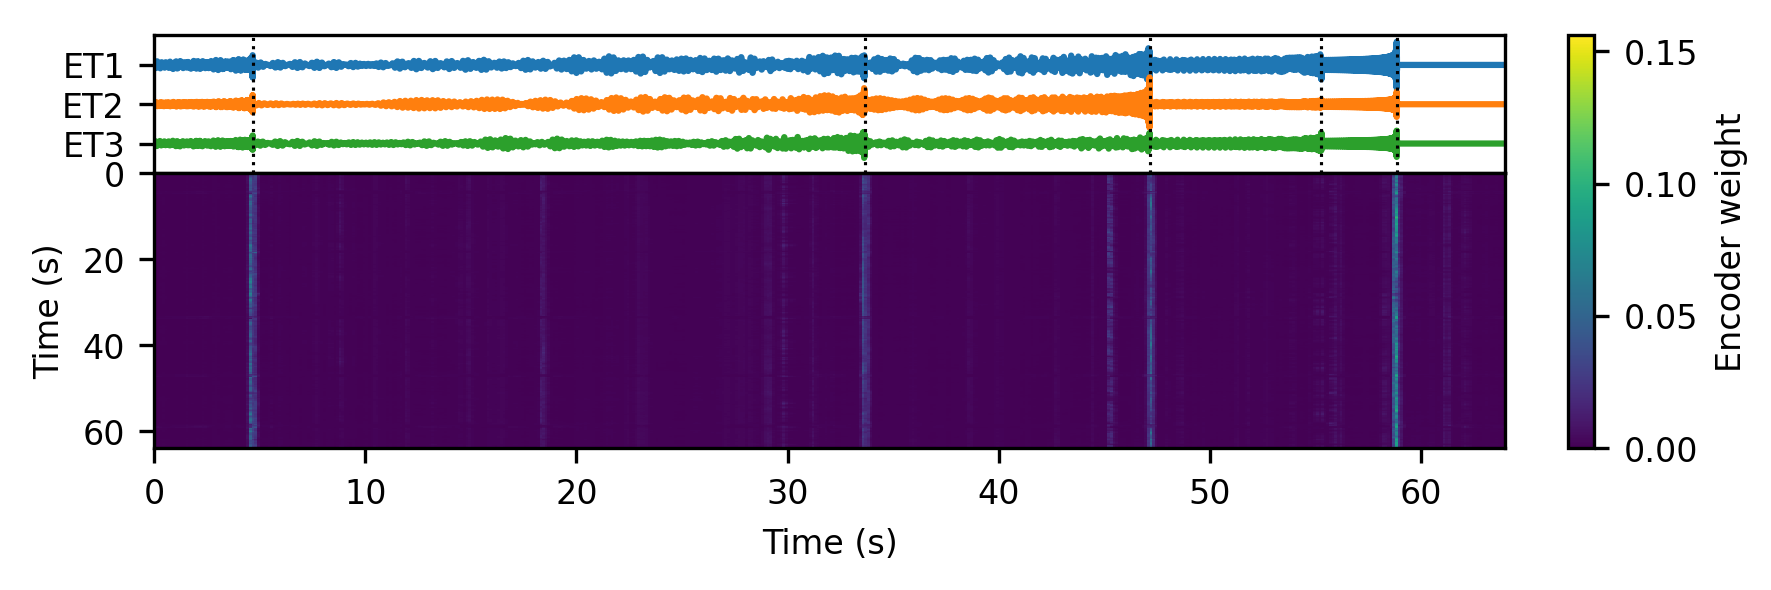
\includegraphics[
	width=15cm,
	]{multiple_signal_detection/plots/weights/encoder/8}
	\caption{Attention matrices of the transformer encoder model for five samples. Each of the $512$ tokens is assigned a time step. The x-axis shows the source sequence tokens and the y-axis the target sequence.}
	\label{fig:heatmap:encoder_weights}
\end{figure}

How the transformer makes use of its large receptive field can be investigated by plotting the encoder attention weights. See the last layer's weights averaged over all attention heads for five samples in Fig.~\ref{fig:heatmap:encoder_weights}. These examples suggest that tokens attend to the identified signals in a sample. It can be concluded that this global information is somehow helpful for making predictions, in high-overlap conditions especially, although it is not fully clear how. 

\section{Injection Study}

It has been seen that the difference in model performance between CNN and transformer encoder is associated with samples containing multiple signals. The results suggest that the CNN's $\approx\SI{1}{\second}$ receptive field is large enough to capture this overlap robustly, but the transformer's \emph{global} receptive field appears to improve performance when dealing with multiple signals per sample $n>1$.
The effect of time overlap is isolated for the case of two signals per sample, $n=2$. Here, according to Fig.~\ref{fig:heatmap:num_mergers}, the transformer encoder outperforms the CNN already with a detection ratio of \SI{63.8(2)}{\percent} compared to \SI{61.2(3)}{\percent}. In particular, model performance is checked against the coalescence-time separation between signals $\Delta t_\text{coa}$ in a controlled injection study. Denoting the two signals A and B, the time separation is defined as $\Delta t_\text{coa}=|t_\text{coa}^\text{A}-t_\text{coa}^\text{B}|$.

% effect of signal closeness on performance
% injection study: multiple datasets, each sample has exactly 2 signals. both injected at fixed times to ensure different delta ts between data sets
% we inject signal B always at 60s and signal A such that delta t is 30s, 10s, 3s, 1s, 0.6s, 0.3s, 0.2s, 0.1s
% these values are approximately logarithmic, with a higher resolution for dt<1s

For this, multiple \SI{66}{\kilo\nothing} sample test-datasets are simulated. What will be referred to as signal B is injected with a fixed coalescence time of \SI{60}{\second}, while signal A is injected at a time $<\SI{60}{\second}$. For each dataset, the signal A injection time is chosen to ensure a constant time separation. A total of eight datasets are simulated with separations of \SI{30}{\second}, \SI{10}{\second}, \SI{3}{\second}, \SI{1}{\second}, \SI{0.6}{\second}, \SI{0.3}{\second}, \SI{0.2}{\second} and \SI{0.1}{\second}. The values are chosen to be equidistant on a logarithmic scale with a higher resolution for $\Delta t_\text{coa}<\SI{1}{\second}$.

\begin{figure}
	\centering
	\makebox[\textwidth]{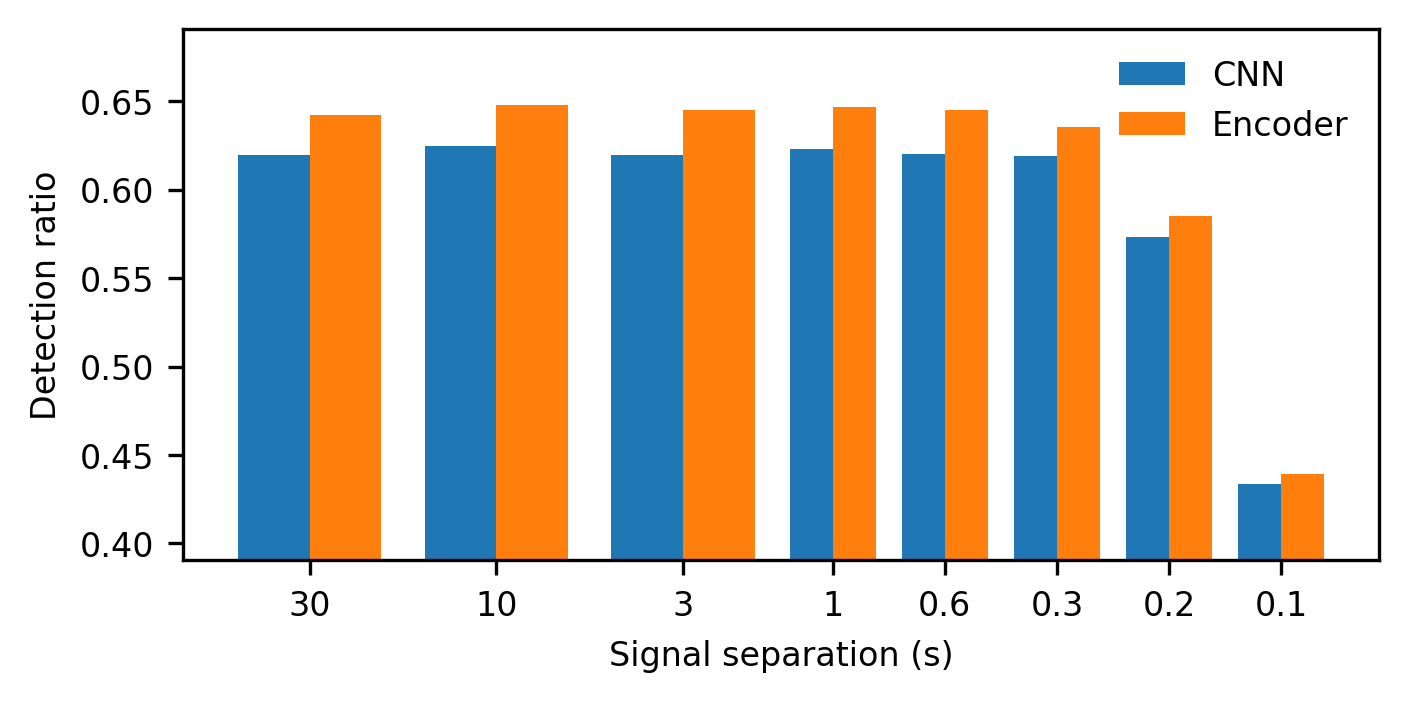
\includegraphics[width=12cm]{multiple_signal_detection/plots/cnn_encoder_deltat}}
	\caption{Detection ratio as a function of signal separation for the CNN (\emph{blue}) and the transformer encoder (\emph{orange}). Computed over \SI{66}{\kilo\nothing} samples with \SI{131}{\kilo\nothing} signals. Uncertainties are too small to be visualized.}
	\label{fig:heatmap:cnn_encoder_deltat}
\end{figure}

% plot detection ratio against signal separation
% two regimes: dt >= 0.3s, performance stays at 61% for cnn and 64% for encoder
% for dt < 0.3, both models degrade and the difference in performance becomes less noticable 
% from this it can be seen that the difference in performance stems not from close overlaps, rather from long range dependencies where the transformers global attention mechanism helps
% As a degradation in performance is noticable for both models once signals get close, it is reasonable to attribute this to the limited heatmap resolution (which is the same in both models)


For both models, the detection ratio is computed over each dataset separately. Assuming a binomial distribution, the uncertainties are $<\SI{0.14}{\percent}$. See the results in Fig.~\ref{fig:heatmap:cnn_encoder_deltat}. From this plot, two regimes can be identified. For $\Delta t_\text{coa} \geq \SI{0.6}{\second}$, model performance is agnostic to signal separation, varying by \SI{0.5(2)}{\percent} at most for the CNN and by \SI{0.6(2)}{\percent} for the encoder. The transformer encoder outperforms the CNN throughout this regime by $\approx\SI{3}{\percent}$. If $\Delta t_\text{coa} \leq \SI{0.3}{\second}$, both models degrade in performance, converging to similar detection ratios of \SI{43.3(1)}{\percent} and \SI{43.9(1)}{\percent}. 

Thus, the difference in model performance does not stem from close overlaps, but rather from long-range dependencies between signals, which are accessible to the transformer model through its global attention mechanism. For small $\Delta t_\text{coa}$, a similar performance decrease is noticeable in both models, suggesting a limitation shared by both architectures, which will be discussed later. 

% study allows for comparison to matched filtering
% \cite{Relton_2022} showed that without adaption matched filtering can handle overlapping signals 
% performance decrease for signals separated by less than 1s, where only one is retained
% see figure, 4 cases
% comparison to encoder model as it is better, this is quantitative only

\begin{figure}
	\centering
	\makebox[\textwidth]{\includegraphics[width=10cm]{multiple_signal_detection/images/delta_tc_stacked_FAR_labels_switched}}
	\caption{Matched-filtering performance as a function of signal separation \cite{Relton_2022}. Four cases are shown: only signal A is recovered (\emph{blue}), only signal B (\emph{red}), both signals (\emph{green}) or neither (\emph{grey}). A denotes the earlier signal.}
	\label{fig:heatmap:matched_filtering_deltat_cases}
\end{figure}

Fig.~\ref{fig:heatmap:cnn_encoder_deltat} shows that both models can detect signals with $\Delta t_\text{coa}\geq\SI{0.6}{\second}$ with no significant performance decrease. In contrast, according to \cite{Relton_2022}, standard matched-filtering searches degrade in performance for signals separated by $<\SI{1}{\second}$ already. In this regime, clustering routines cause only one of the two signals to be recovered. This injection study allows for a more direct comparison with matched filtering, as the methodology is similar to \cite{Relton_2022}. See their results in Fig.~\ref{fig:heatmap:matched_filtering_deltat_cases}. 
Because the exact datasets differ in signal parameters and SNRs and different FARs are employed, comparisons will be \emph{qualitative} only. 

\begin{figure}
	\centering
	\makebox[\textwidth]{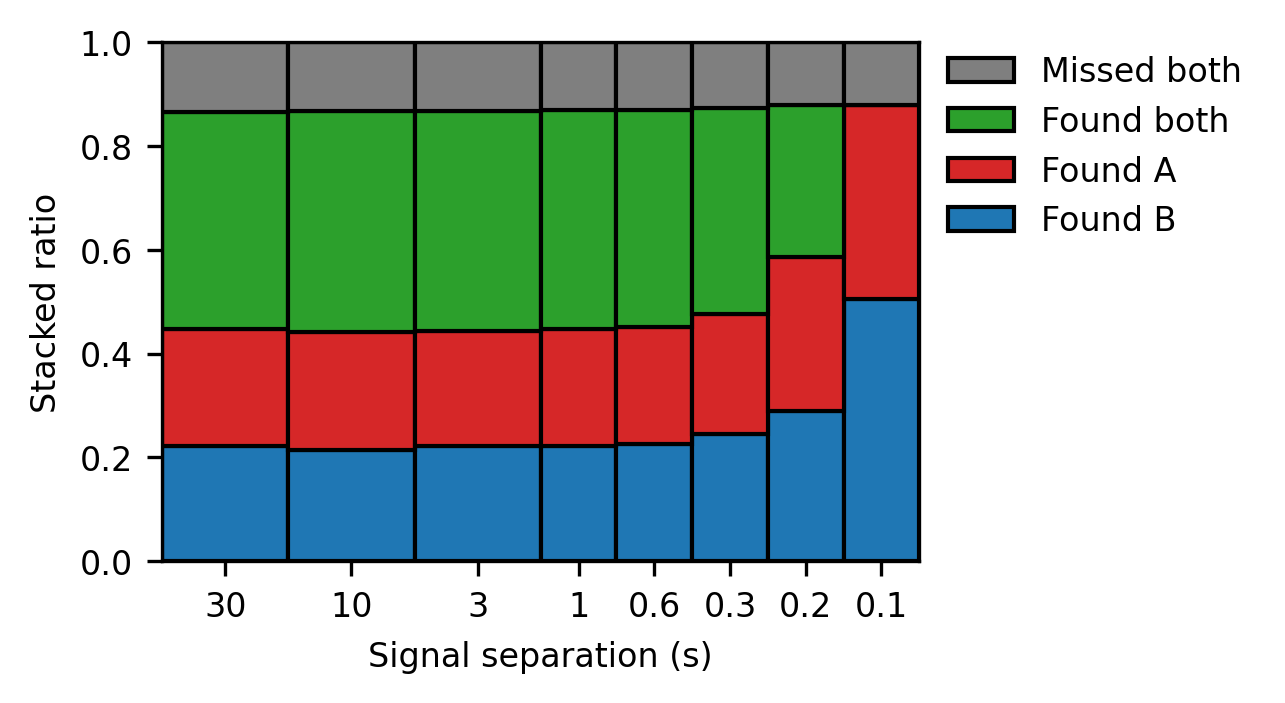
\includegraphics[width=11cm]{multiple_signal_detection/plots/encoder_stacked}}
	\caption{Transformer encoder performance with signal separation. For comparison with Fig.~\ref{fig:heatmap:matched_filtering_deltat_cases}, notice the different x-axis scale.}
	\label{fig:heatmap:encoder_deltat_cases}
\end{figure}

Fig.~\ref{fig:heatmap:matched_filtering_deltat_cases} is reproduced for the transformer encoder by distinguishing four cases: the model finds only signal A, only signal B, both signals or neither. Because comparisons are qualitative anyway, uncertainties are  simply neglected here. See the results in Fig.~\ref{fig:heatmap:encoder_deltat_cases}.
The plot shows that the model can distinguish signals up to separations of $\SI{0.2}{\second}$. At $\Delta t_\text{coa}=\SI{0.1}{\second}$, only one of two signals is recovered. Thus, at least qualitatively, the transformer encoder model is more robust than standard matched-filtering searches when handling close overlaps. 

\begin{figure}
	\centering
	\makebox[\textwidth]{
		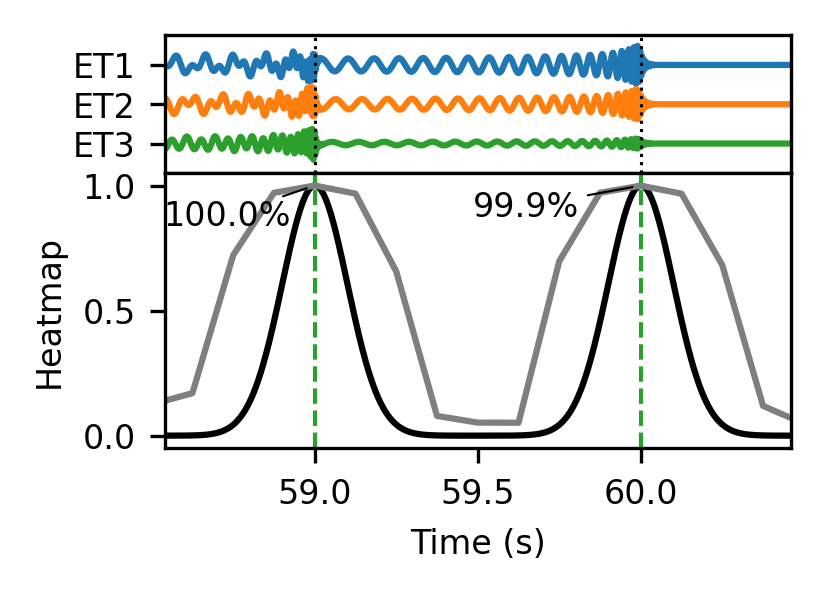
\includegraphics[
		height=5cm,
		trim=0 0 0 0,
		clip
		]{multiple_signal_detection/plots/out/700/encoder/0_zoom}
		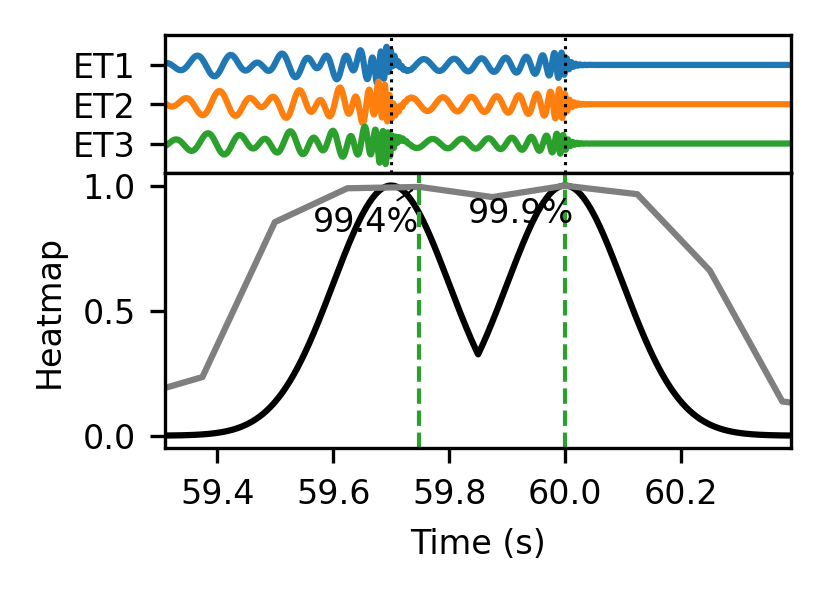
\includegraphics[
		height=5cm,
		trim=1.2cm 0 0 0,
		clip
		]{multiple_signal_detection/plots/out/800/encoder/7_zoom}
		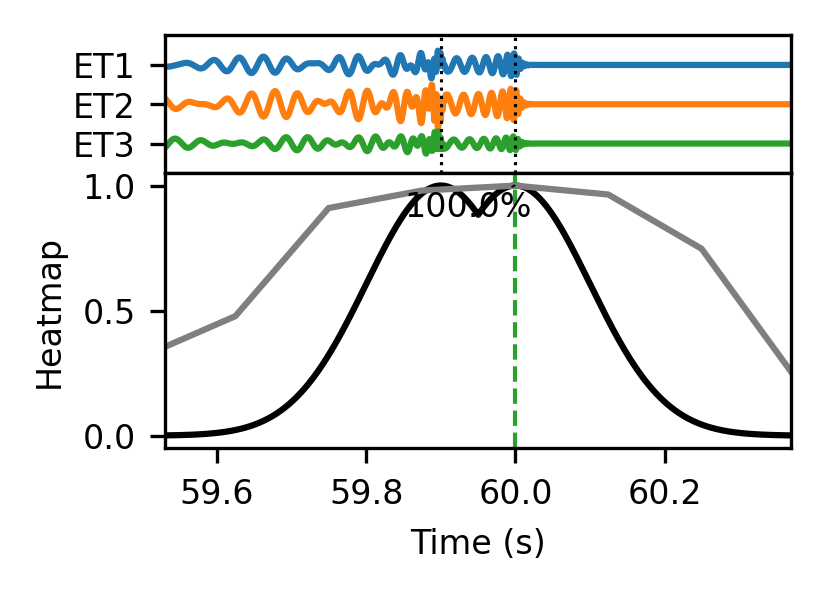
\includegraphics[
		height=5cm,
		trim=1.2cm 0 0 0,
		clip
		]{multiple_signal_detection/plots/out/900/encoder/6_zoom}
	}
	\caption{Three example ground-truth (\emph{black}) and predicted heatmaps (\emph{grey}) of the transformer encoder model for $\Delta t_\text{coa}=\SI{1}{\second}$ (\emph{left}), $\Delta t_\text{coa}=\SI{0.3}{\second}$ (\emph{middle}) and $\Delta t_\text{coa}=\SI{0.1}{\second}$ (\emph{right}).}
	\label{fig:heatmap:encoder_deltat_plot}
\end{figure}

As previous results suggest a limitation in both the CNN and encoder architectures for $\Delta t_\text{coa}\leq\SI{0.3}{\second}$, it is reasonable to attribute the performance decrease in this regime to the limited heatmap time resolution.  
Because of downsampling, heatmaps comprise $512$ time steps only, resulting in a sample time of \SI{0.125}{\second}. Thus, if two signals are separated by less than \emph{two} time steps, $\Delta t_\text{coa}<\SI{0.25}{\second}$, the resulting heatmap prediction can only produce one peak. See example ground-truth and predicted heatmaps in Fig.~\ref{fig:heatmap:encoder_deltat_plot}.

\section{Summary}

% heatmap regression for multiple overlapping signals

This chapter reformulated GW detection as a heatmap regression task. Adaptations have been made to the approach in previous research \cite{PhysRevD.100.063015} to reduce the number of post-processing steps and to handle multiple signals per sample.

% comparison of two models, one CNN (more standard) and one transformer (motivated by \cite{Papalini_2025})
% transformer outperforms CNN because it can handle long range dependencies through attention mechanism

Two architectures were investigated: a CNN and a transformer encoder, which were adapted from the binary-classification models introduced previously. Both achieved low FARs down to $1/\SI{}{\month}$ while retrieving a non-zero fraction of signals, with the transformer consistently outperforming the CNN.

An injection study showed that this advantage does not arise from resolving closely overlapping signals, but from exploiting long-range dependencies between multiple signals. Both architectures exhibited a common performance limit for signal separations $\leq\SI{0.3}{\second}$, consistent with the resolution of the predicted heatmaps. 

% models are better at handling close overlaps (qualitatively) than matched filtering
% struggle for dt<=0.3s because of heatmap resolution
% look into upsampling like unet?
